\chapter{Relationship among  $B_1$-EPG, EPT and VPT graph classes}
\label{cap:v}

\begin{flushright}
\begin{minipage}[t][0cm][b]{0.47\textwidth}
\emph{
A Matemática não mente. Mente quem faz mau uso dela.}
\end{minipage}

\rule[0cm]{7cm}{0.03cm}%{largura}{espessura}

Albert Einstein
\end{flushright}

This chapter presents as a main result that every Chordal $B_1$-EPG graph is simultaneously in the VPT and EPT graph classes. In particular, we describe structures that are always present in graphs that do not support a Helly-$B_1$-EPG representation and thus we define some sets of subgraphs that delimit Helly subfamilies. 
 In addition, this chapter also features characterizations for some non-trivial graph families that are properly contained in Helly-$B_1$ EPG, namely these families are composed of the Bipartite, Blocks, Cactus and Line of Bipartite  graphs.



\section{Introduction}

Models based on paths intersection  may consider  intersections by vertices or   intersections by edges.  Cases where the paths are hosted on a tree  appear first in the literature, see for instance \cite{gavril1978recognition, golumbic1985edge, golumbic1985}.  Representations using paths on a grid were considered later, see  \cite{golumbic2009,golumbic2013, golumbic2013intersection}. %More details on each intersection model will be given in the following text.

 Let $P$ be a family of paths on a host tree $T$ . Two types of intersection graphs from the pair $<P,T>$ are defined, namely VPT and EPT graphs.
The \textit{edge intersection graph} of $P$, EPT(P), has vertices which correspond to the members of $P$, and two vertices are adjacent in EPT(P) if and only if the corresponding paths in $P$ share at least one edge in T. Similarly, the \textit{vertex intersection graph} of $P$, VPT(P), has vertices which correspond to the members of $P$, and two vertices are adjacent in VPT(P) if and only if the corresponding paths in $P$ share at least one vertex in $T$.
%
VPT and EPT graphs are incomparable families of graphs. However, when the maximum degree of the host tree is restricted to three the family of
VPT graphs coincides with the family of EPT graphs \cite{golumbic1985edge% \cite{alcon2010necessary
}. Also it is known that any Chordal EPT graph is VPT (see~\cite{syslo1985triangulated}). Recall that it was shown that Chordal graphs are the vertex intersection graphs of subtrees of a tree \cite{gavril1974intersection}.


Edge intersection graphs of paths on a grid are called \textit{EPG graphs}. 

In \cite{golumbic2009}, the authors proved that every graph is EPG, and started the study of the subclasses
defined by bounding the number of times any path used in the representation can bend.  Graphs admitting a representation
where  paths  have at most $k$ changes of direction  (bends) were called $B_k$-EPG. 
 In particular, when the paths have at most one bend we have the \textit{ $B_1$-EPG graphs} or a \textit{single bend EPG graphs}.

 A pertinent question in the context of path intersection graphs is as follows: given two classes of path intersection graphs,
 the first whose host is a tree and the second whose host is a grid,  is there an intersection or containment relationship among these classes? What do we know about it?

In the present chapter we will explore $B_1$-EPG graphs, in particular diamond-free graphs and Chordal graphs. We will work on the question about the containment relation between  VPT, EPT and $B_1$-EPG graph classes.


 A collection  of sets satisfies the \textit{Helly property} when every pair-wise intersecting sub-collection  has at least one common element. When this property
 is satisfied by the set of vertices (edges) of the paths used in a representation, we get a Helly representation.  Helly-$B_1$-EPG graphs were studied
 in \cite{bornstein2019, dmtcs:6506}.                                     
It is known that not every $B_1$-EPG graph admits a Helly-$B_1$-EPG representation. We are interested in determining the subgraphs that make
$B_1$-EPG graphs do not admit a Helly representation. In the present chapter, we describe some structures that will be present in any such subgraph,
and, in addition, we present new  Helly-$B_1$ EPG  subclasses.
Moreover,  we  describe new  Helly-$B_1$ EPG  subclasses % that have Helly property 
and we give some sets of subgraphs that delimit Helly subfamilies.   
\section{Definitions and Technical Results}

The \textit{vertex set} and the \textit{edge set} of a graph $G$ are denoted by $V(G)$ and $E(G)$, respectively.  Given a vertex $v\in V(G)$,  $N(v)$ and $N[v]$ represent the open and the close
 \textit{neighborhood} of $v$ in $G$, respectively. 
For a subset $S \subseteq V(G)$,  $G[S]$ is the subgraph of $G$ induced by $S$.
 If $\mathcal{F}$ is any family of graphs, we say that  $G$ is  \textit{$\mathcal{F}$-free} if $G$ has no induced subgraph isomorphic to a member of $\mathcal{F}$.
 A \textit{cycle},  denoted by $C_n$,  is a sequence of distinct
vertices $v_1, \dots , v_n, v_1$  where $v_i \neq v_j$ for $i \neq j$ and $(v_i, v_i + 1) \in E(G)$, such that
$n \geq 3$. A \textit{chord} is an edge that is between two non-consecutive vertices in a sequence of vertices of a cycle. An \textit{induced cycle}  or \textit{chordless cycles} is a cycle that has no chord, in this paper an induce cycle will simply be called  \textit{cycle}. A graph $G$ formed by an induced cycle $H$ plus  a single universal vertex $v$ connected to all vertices of $H$
is called \textit{wheel graph}. If the wheel has $n$ vertices, it is denoted by $n$-wheel. 

The $k$\textit{-sun graph }$S_k$, $k \geq 3$, consists of
$2k$ vertices, an independent set $X = \{x_1, \dots, x_k\}$ and a clique $Y = \{y_1, \dots, y_k\}$, and edges set $E_1 \cup E_2$, where $E_ 1=\{ (x_1,y_1); (y_1, x_2); (x_2, y_2); (y_2, x_3); \dots , (x_k, y_k); (y_k, x_1) \}$ forms the outer cycle and $E_2= \{(y_i, y_j) |i\neq j\}$ forms the inner clique.

A graph is a $ B_k$-EPG graph if it admits an EPG representation in which each path has at most $k$ bends.  When $ k = 1 $ we say that this is a \emph{single bend EPG} representation or simply a $B_1$-EPG representation.
A \textit{clique} is a set of pairwise adjacent vertices and
an \textit{independent set} is a set of pairwise non adjacent vertices.
Given an EPG representation of a graph $G$, we will identify each vertex $v$ of $G$ with the corresponding path $P_{v}$ of the grid used in the representation. Accordingly, for instance, we will say that a vertex of $G$ covers or contains some edge of the grid (meaning that the corresponding path does), or that a set of paths of the representation
induces a subgraph of $G$ (meaning that the corresponding set of vertices does). 

In  a $B_1$-EPG representation, a clique $K$  is said to be
 an \textit{edge-clique} if all the vertices of $K$ share a common edge of the grid (see Figure~\ref{fig:cliquesRepresentation}(a)).
 A \textit{claw of the grid} is a set of three edges of the grid incident into a same point of the grid, which is called
  the \textit{center of the claw}. The two edges of the claw that have the same direction form
    the \textit{ base of the claw}. If $K$ is not an edge-clique, then there exists
    a claw of the grid (and only one) such that the vertices of $K$ are those containing exactly two of the three edges of the claw; such a  clique is called  \textit{claw-clique} \cite{golumbic2009} (see Figure~\ref{fig:cliquesRepresentation}(b)).

    

\begin{figure}[h]
  \centering
  \begin{tabular}{  p{4.5cm} p{0.7cm} p{4cm} }
    %\centering
    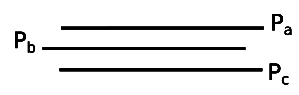
\includegraphics[width=4.5cm]{img/edge-clique.png} & &
    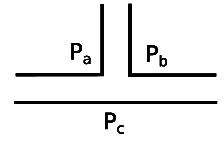
\includegraphics[width=3.5cm]{img/claw-clique.png}%b1EpgTransparenteGrade2
    \\
    \footnotesize %\centering 
    (a)  \footnotesize Representation of a clique as edge-clique. && \footnotesize (b) Representation  of a clique as claw-clique.\\
  \end{tabular}

 \caption{Examples of clique representations.} \label{fig:cliquesRepresentation}
\end{figure}


















% \begin{figure}[h]
%   \centering
%   \begin{tabular}{  p{4cm} p{0.7cm} p{4cm} }
%     %\centering
%     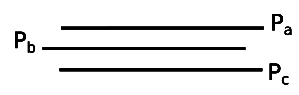
\includegraphics[width=4.5cm]{img/edge-clique.png} & &
%     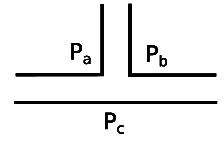
\includegraphics[width=3.5cm]{img/claw-clique.png}%b1EpgTransparenteGrade2
%     \\
%     \footnotesize %\centering 
%     (a)  \footnotesize Representação de uma  clique como clique-aresta. && \footnotesize (b) Representação de uma  clique como clique-garra.\\
%   \end{tabular}

%  \caption{Exemplos de representações de clique.} \label{fig:cliquesRepresentation}
% \end{figure}    

Notice that if three vertices induce a claw-clique, then exactly two of them turn at the center of the corresponding  claw of the grid, and the third one contains the
base of the claw. 
Furthermore, any other vertex  adjacent to the three  must contain two of the edges of that claw, then the following lemma holds.

\begin{lema}\label{lem:cliquesMaximais}
If three vertices are together  in more than one maximal clique of a graph $G$, then in
any $B_1$-EPG representation of $G$ the three vertices do not form a claw-clique. %corresponding paths do not form a claw.
\end{lema}

\begin{figure}[ht]
  \centering
  \begin{tabular}{  p{5cm} p{0.7cm} p{5cm} }
    %\centering
    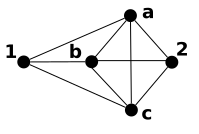
\includegraphics[width=3.5cm]{img/lemaClaw2Maximais} & &
    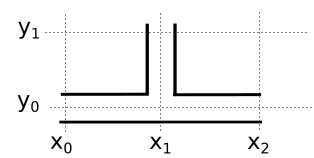
\includegraphics[width=5.5cm]{img/claw2}
    \\
    \footnotesize %\centering 
    (a)  \footnotesize Examplo de duas cliques maximais compartilhando vértices. && \footnotesize (b) Representação de uma clique-garra na grade.\\
  \end{tabular}

 \caption{Vértices representados por uma garra  estão presentes em uma única clique maximal.} \label{fig:lemaClaw2Maximais}
\end{figure}

In \cite{ries2009} Asinowski et al. proved the following lemma for $C_4$-free graphs.

\begin{lema} \cite{ries2009} \label{lem:lemaBRies2009}
Let $G$ be a $B_1$-EPG graph. If $G$ is $C_4$-free, then there exists a $B_1$-EPG representation of $G$ such that every  maximal claw-clique $K$ is represented on a claw of the grid whose base is covered only by vertices of $K$.
\end{lema}


We have obtained the following similar result for diamond-free graphs. A \textit{diamond} is a graph $G$ with vertex set $V(G) = \{a, b, c, d\}$ and edge set $E(G)=\{ab, ac,bc, bd,cd\}$ (see Figure~\ref{fig:diamond}). %A graph is diamond-free if it does not contain a diamond as induced subgraph.

 \begin{figure}[htb]	
 \center%6.3
 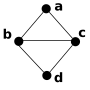
\includegraphics[width=2.2cm]{./img/diamond.png}
 \caption{Diamond graph.}
\label{fig:diamond}
\end{figure}  
 


\begin{lema}\label{lem:b1epgDiamondFree}
Let $G$ be a $B_1$-EPG graph. If $G$ is diamond-free, then in any $B_1$-EPG representation of $G$,  every maximal claw-clique $K$ is represented on a claw of the grid whose edges are covered only by vertices of $K$.
\end{lema}

\begin{proof}Let $K$ be a maximal clique which is a claw-clique in a given $B_1$-EPG representation of $G$. Then there exist three vertices of $K$ which induce a claw-clique $K'$ on
the same claw of the grid than $K$. Assume, in order to derive a contradiction, that a vertex $v\notin K$ covers some edge of the claw. Clearly, $v$ must  cover
only one of such edges. Therefore $v$ and the vertices of $K'$ induce a diamond, a contradiction. 
\end{proof}


% \begin{defi} \label{defi:tortasFrame}

Let $ Q $ be a grid and let $ (a_1, b),$ $(a_2, b),$ $(a_3, b),$ $(a_4, b)$ be a $4$-star centered at $b$ as depicted in Figure~\ref{fig:piesInGrid}(a). Let $ \mathcal{P} = \{P_1, \dots , P_4\}$ be a collection of four paths each containing a different pair of edges of the $4$-star.
%exactly two edges of the $4$-star:
Following \cite{golumbic2009}, we say that the four paths form
\begin{itemize}
\item a \emph{true pie} %is a representation where each $P_i$ of $ \mathcal{P} $ has a bend at $b$.
when each one has a bend at $b$, Figure~\ref{fig:piesInGrid}(b); and 
\item a \emph {false pie} when exactly two of the paths %$P_i$  do not 
bend at $b$ and they do not share an edge of the $4$-star, Figure~\ref{fig:piesInGrid}(c). %contain bends, while the remaining two do not share an edge. 

\begin{figure}[htb]
  \centering
%segundo bloco de figuras
  \begin{tabular}{c c c c c }
    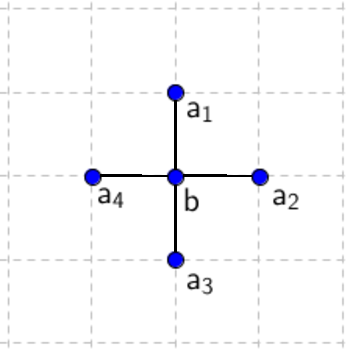
\includegraphics[width=3.5cm]{img/disposicaoTortaGrid3.pdf}    
    & &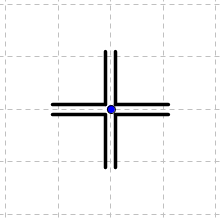
\includegraphics[width=3.5cm]{img/truePieGrid} 
    & &
 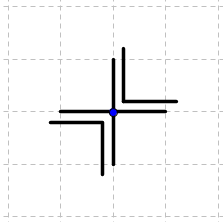
\includegraphics[width=3.5cm]{img/falsePieGrid} \\%[\abovecaptionskip]
    {\footnotesize (a) 4-estrela em uma grade.}  & &  {\footnotesize (b) Torta verdadeira.} & & {\footnotesize (c) Torta falsa.} 
  \end{tabular}
  \caption{Representação $B_{1}$-EPG do ciclo induzido de tamanho  4 como tortas, com ênfase no centro $b$.}\label{fig:piesInGrid}
\end{figure} 

%\vspace{-0.5cm}
\end{itemize}
% \end{defi}

Clearly if four paths of a $B_1$-EPG representation of $G$ form a pie, then the corresponding vertices induce a $4$-cycle in $G$. % The converse implication is also true (see~\cite{golumbic2009}). 
The following result can be easily proved. We say that a set of paths form a claw when each pair of edges of the claw is covered by some of the paths.

\begin{lema}\label{lem:twoClawNotSameCenterInChordal}
In any $B_1$-EPG representation of a graph $G$, a set of paths forming two different claws centered at the same point of the grid contains four paths forming either a true pie or a false pie. Therefore, in any $B_1$-EPG representation of a chordal graph $G$, no two maximal claw-cliques of $G$ are centered at the same point of the grid.
\end{lema}

\begin{lema}\label{lem:3cliquesNotClaw}
Let $G$ be a graph whose vertex set  can be
partitioned into a non trivial clique $K$ and an independent set $I=\{w_1,w_2,w_3\}$, such that each vertex of $K$ is adjacent to each vertex of $I$. Then, in any $B_1$-EPG representation of $G$, at least one of the cliques  $K_i = K \cup \{w_i\}$, with $1 \leq i \leq 3$,  is an edge-clique. 
\end{lema}

\begin{proof}
Assume, in order to derive a contradiction, that the three cliques are claw-cliques. By Lemma~\ref{lem:twoClawNotSameCenterInChordal}, they have different centers, say the points $q_1, q_2, q_3$ of the grid, respectively. Since at least two paths have a bend at the center of a claw, for each $i\in\{1,2,3\}$,   there must exist a vertex
  $v_i$ of $K$ such that the corresponding path $P_{v_i}$ turns at the point $q_i$ of the grid.  Notice that each one of the three paths $P_{v_i}$
  must contain  the three grid points $q_1$, $q_2$ and $q_3$. To prove that this is not possible, we will consider, without loss of generality, two cases.
  First,  $q_1$ is between $q_2$ and $q_3$ in $P_{v_1}$. Then, $P_{v_3}$ cannot turn at $q_3$ and contain $q_1$ and $q_2$.   And second,
  $q_2$ is between $q_1$ and $q_3$ in $P_{v_1}$. In this case, $P_{v_2}$ cannot turn at $q_2$ and contain $q_1$ and $q_3$; thus the proof is completed.
 
\end{proof}

Three vertices $u, v, w$ of a graph $G$ form an \textit{asteroidal triple} (AT) of $G$ if for every pair of them there exists a path connecting the two vertices and such that the path avoids the neighborhood of the remaining vertex~\cite{Asinowski2009}. A graph without an asteroidal triple is called \textit{AT-free}. 

\begin{lema}
[\cite{ries2009}] \label{l:AT-free} Let $v$ be any vertex of a $B_1$-EPG graph $G$. Then $G[N(v)]$ is AT-free.
\end{lema}

Let $C$ be any subset of the vertices of a graph $G$. The \textit{branch graph} $B(G|C)$, see~\cite{golumbic2009}, of $G$ over $C$ has a vertex set, $V(B)$, consisting of all the vertices of $G$ not in $C$ but adjacent to some member of $C$, i.e. $V(B) = N(C) - C$. Adjacency in $B(G|C)$ is defined as follows: we join two vertices $x$ and $y$ by an edge in $E(B)$ if and only if in $G$ occurs:
\begin{enumerate}
    \item  $x$ and $y$ are not adjacent;
    \item $x$ and $y$ have a common neighbor $u \in C$;
    \item the sets $N(x) \cap C$ and $N(y) \cap C$ are not comparable, i.e. there exist private neighbors $w, z \in C$ such that $w$ is adjacent to $x$ but not to $y$, and $z$ is adjacent to $y$ but not to $x$; we say that $x$ and $y$ are neighborhood incomparable.
\end{enumerate}

A graph $G$ is \textit{k-colorable} if its vertices can be colored with at most $k$ colors in such a way that no two adjacent vertices share the same color. 

\begin{lema}[~\cite{golumbic2009}] \label{l:branch} Let $C$ be any maximal clique of a $B_1$-EPG  graph $G$. Then, the branch graph $B(G|C)$ is $\{P_6, \, C_n \hbox{ for }  n\geq 4\}$-free.
\end{lema}







\section{Subclasses of Helly-$B_1$-EPG Graphs}

In this section, we delimit some  subclasses of $B_1$-EPG graphs that admit a Helly-$B_1$-EPG representation. It is known that $B_1$-EPG and Helly-$B_1$ EPG 
are hereditary classes, so they can  be characterized by forbidden structures. 
In both cases, finding the list of minimal forbidden induced subgraphs are challenging open problems.
Taking a step towards solving
those problems,  we describe a few structures % that  provide a $B_1$-EPG graph does not admit a Helly-$B_1$ EPG representation, that is it is not a  Helly-$B_1$ EPG graph. 
at least one of which will  necessarily be present in  any $B_1$-EPG graph that does not admit a Helly representation. 
In addition,
we show that the well known families of Block graphs, Cactus and Line of Bipartite graphs are totally contained in the class Helly-$B_1$ EPG.


Let $S_{3}, S_{3'}, S_{3''}$ and $ C_{4}$ be the graphs depicted in Figure \ref{fig:proibidos}. 


\begin{theorem}
\label{lem:chordalDiamondFree}
Let $G$ be a $B_1$-EPG graph. If $G$ is  $\{S_{3}, S_{3'}, S_{3''}, C_{4}\}$-free then $G$  is a Helly-$B_1$-EPG graph.
\end{theorem}

\begin{proof}
If $G$ is not a Helly-$B_1$-EPG graph, then in each $B_1$-EPG representation of $G$, there is at least one clique that is represented as claw-clique and no as edge-clique. Consider any $B_1$-EPG  representation of $G$  and let $K$ be a maximal clique  which is represented as a claw-clique. Assume, w.l.o.g,  $K$ is on a claw of the grid with base $[x_0, x_2]\times\{y_0\}$ and center $C = (x_1, y_0)$. Denote by  $\mathcal{P}_K$ the set of paths corresponding to the vertices of $K$.  By Lemma~\ref{lem:lemaBRies2009},  %(see~\cite{ries2009})
%no path $P_w$ for $w\notin K$ covers 
the grid segment $[x_0, x_2]\times\{y_0\}$ is covered only by vertices of $K$. % because $G$ is $C_4$-free


 For every ${\displaystyle \lrcorner}$-path %$P_v \in \mathcal{P}_K$ 
 (resp. ${\displaystyle \llcorner}$-path 
% $P_{v'} \in \mathcal{P}_K$
 ) belonging to $\mathcal{P}_K$, we do the following: if %$P_v$ (resp. $P_{v'}$)
 the path does not intersect any path $P_t \notin\mathcal{P}_K$ on column $x_1$, then we delete its vertical segment and add the grid segment $[x_1, x_2]\times\{y_0\}$ (resp. $[x_0, x_1]\times\{y_0\}$). If after this transformation there is no more ${\displaystyle \lrcorner}$-paths (resp. ${\displaystyle \llcorner}$-paths) in $\mathcal{P}_K$, then we are done since we have obtained an edge-clique. So we may assume that
 every ${\displaystyle \lrcorner}$-path   and every ${\displaystyle \llcorner}$-path  in $ \mathcal{P}_K$ intersects some path $P_t \notin \mathcal{P}_K$   on column $x_1$ (notice that we can assume is the same path $P_t$ for all the vertices). 
 
 Now, if none of the ${\displaystyle \lrcorner}$-paths belonging to $\mathcal{P}_K$ intersects  a path non in  $ \mathcal{P}_K$ on the line $y_0$, then we can replace the horizontal part of those paths by the segment $[x_1,x_2]\times \{y_0\}$, getting an edge representation of the clique $K$. Thus, we can assume there exists
 at least one ${\displaystyle \lrcorner}$-path $P_{v} \in \mathcal{P}_K$ intersecting some path  $P_{t'} \notin \mathcal{P}_K$ on line $y_0$. Analogously, there exists
 at least one ${\displaystyle \llcorner}$-path $P_{v'} \in \mathcal{P}_K$ intersecting some path  $P_{t''} \notin K$ on line $y_0$, as depicted in Figure~\ref{fig:clawGrid}. Notice that vertex $t'$ cannot be adjacent to any of the vertices $t$, $v'$ or $t''$; and, in addition, vertex $t''$ cannot
 be adjacent to   $t$,  or $v$.
 
 Finally,   since $K$ is claw-clique,  there is a path $P_u \in \mathcal{P}_K$ covering the base of the claw. Depending on the 
 possibles adjacencies between  $u$ and $t'$ or  $t''$, one of the graphs  $S_{3}$, $S_{3'}$ or $S_{3''}$ is obtained.

\end{proof}



\begin{figure}[h]
  \centering
  \begin{tabular}{  c p{0.7cm} c}
    %\centering
    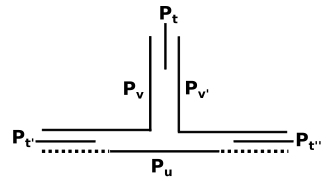
\includegraphics[width=5.5cm]{img/clawGrid} & &
    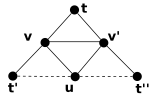
\includegraphics[width=3.5cm]{img/clawInduced.png}
    \\
    \footnotesize %\centering 
    (a)  \footnotesize Claw with paths. && \footnotesize (b) Subgraph induced by paths.\\
  \end{tabular}

 \caption{Reconstruction of the intersection model.}
 \label{fig:clawGrid}
\end{figure} 

 


% \begin{figure}[h]
%   \centering
%   \begin{tabular}{  c p{0.7cm} c}
%     %\centering
%     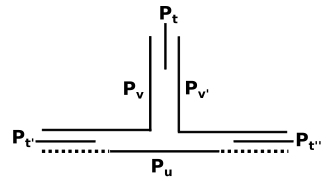
\includegraphics[width=5.5cm]{img/clawGrid} & &
%     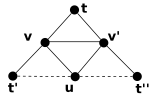
\includegraphics[width=3.5cm]{img/clawInduced.png}
%     \\
%     \footnotesize %\centering 
%     (a)  \footnotesize Clique-garra com caminhos adicionais. && \footnotesize (b) Subgrafo induzido pelos caminhos.\\
%   \end{tabular}

%  \caption{Reconstrução do modelo de intersecção.}
%  \label{fig:clawGrid}
% \end{figure} 

 



Notice that any bull-free graph is $\{S_{3}, S_{3'}, S_{3''}\}$-free, so our previous result implies  Lemma 5 of  \cite{ries2009}.


\begin{figure}[h]
  \centering
  \begin{tabular}{  c p{0.7cm} c }
    \centering
    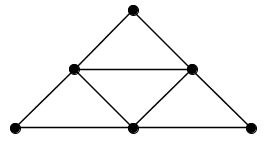
\includegraphics[width=4cm]{img/s3.png} & &
    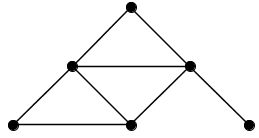
\includegraphics[width=4cm]{img/s3-1.png}
    \\
    \footnotesize \centering 
    (a)  \footnotesize Grafo $S_3$. &&  \footnotesize (b) Grafo $S_{3'}$. \\
    
    %---------------------
      \centering 
      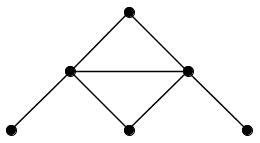
\includegraphics[width=4cm]{img/s3-2.png} & &
    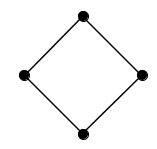
\includegraphics[width=3cm]{img/c4.png}
    \\
    \footnotesize \centering 
    (c)  \footnotesize Grafo $S_{3''}$. && \footnotesize (b) Grafo $C_{4}$.\\
  \end{tabular}

 \caption{Grafos do enunciado do  Teorema~\ref{lem:chordalDiamondFree}.}
 \label{fig:proibidos}
\end{figure} 



%--------------------------


Next theorem has as consequence the identification of several graph classes where the existence of a $B_1$-EPG representation ensures the existence of a Helly-$B_1$-EPG representation.


\begin{theorem} \label{lem:b1DiamondFree}
 If $G$ is a $B_1$-EPG and diamond-free graph then $G$ is a Helly-$B_1$-EPG graph.
 \end{theorem}

\begin{proof}
If $G$ is not a Helly-$B_1$-EPG graph, then in each $B_1$-EPG representation of $G$, there is at least one clique that is represented as claw-clique and no as edge-clique.  Consider any $B_1$-EPG  representation of $G$  and let $K$ be a maximal clique  which is represented as a claw-clique. Assume, w.l.o.g,  $K$ is on a claw of the grid with base $[x_0, x_2]\times\{y_0\}$ and center $C = (x_1, y_0)$. Denote by  $\mathcal{P}_K$ the set of paths corresponding to the vertices of $K$. 
 By Lemma~\ref{lem:b1epgDiamondFree},  %(see~\cite{ries2009})
%no path $P_w$ for $w\notin K$ covers 
the grid segment $[x_0, x_2]\times\{y_0\}$ is covered only by vertices of $K$. % because $G$ is $C_4$-free
 For every ${\displaystyle \lrcorner}$-path %$P_v \in \mathcal{P}_K$ 
 (resp. ${\displaystyle \llcorner}$-path 
% $P_{v'} \in \mathcal{P}_K$
 ) belonging to $\mathcal{P}_K$, we do the following: if %$P_v$ (resp. $P_{v'}$)
 the path does not intersect any path $P_t \notin\mathcal{P}_K$ on column $x_1$, then we delete its vertical segment and add the grid segment $[x_1, x_2]\times\{y_0\}$ (resp. $[x_0, x_1]\times\{y_0\}$). If after this transformation there is no more ${\displaystyle \lrcorner}$-paths (resp. ${\displaystyle \llcorner}$-paths) in $\mathcal{P}_K$, then we are done since we have obtained an edge-clique. So we may assume that
 every ${\displaystyle \lrcorner}$-path   and every ${\displaystyle \llcorner}$-path  in $ \mathcal{P}_K$ intersects some path $P_t \notin \mathcal{P}_K$   on column $x_1$ (notice that we can assume is the same path $P_t$ for all the vertices). Since  $K$ is claw-clique,  there is a path $P_u \in \mathcal{P}_K$ covering the base of the claw. Thus, $G[v, v', u, t]$ induces a diamond,  a contradiction. 
\end{proof}  

An \textit{independent set} of vertices is a set of vertices no two of which are adjacent.
A graph $G$ is said to be \textit{Bipartite} if its set of vertices can be partitioned into two distinct independent sets.
 There are Bipartite graphs that are non $B_1$-EPG, for instance $K_{2,5}$ and $K_{3,3}$ (see~\cite{cohen2014}). Clearly , since
 bipartite graphs are triangle-free, any $B_1$-EPG representation of a bipartite graph is also a Helly-$B_1$-EPG representation.
 A similar result (but a bit weaker) is obtained as corollary of the previous theorem. 


\begin{corollary}
If $G$ is a Bipartite $B_1$-EPG graph then $G$ is a Helly-$B_1$-EPG graph.
\end{corollary}

\begin{proof}
The Bipartite graphs are diamond-free, thus by Theorem~\ref{lem:b1DiamondFree} these graphs are Helly-$B_1$-EPG graphs.
\end{proof}

A \textit{Block graph} or \textit{Clique Tree} is a type of graph in which every biconnected component (block) is a clique.

\begin{corollary}\label{lem:cdf}
 Block graphs are Helly-$B_1$ EPG.
\end{corollary}

\begin{proof}
Block graphs are known to be exactly the chordal diamond-free graphs, so by   Theorem 19 of \cite{ries2009}, all Block graphs are  $B_1$-EPG. If follows from Theorem~\ref{lem:b1DiamondFree} that all Block graphs are Helly-$B_1$ EPG. 
 \end{proof} 

A \textit{Cactus} (sometimes called a cactus tree)  graph is a connected graph in which any two  cycles have at most one vertex in common. Equivalently, it is a connected graph in which every edge belongs to at most one  cycle, or (for nontrivial cactus) in which every block (maximal subgraph without a cut-vertex) is an edge or a cycle. The family of graphs in which each component is a cactus is closed under graph minor operations. This graph family may be characterized by a single forbidden minor, the diamond graph.
 
\begin{corollary}
Cactus graphs are  Helly-$B_1$ EPG.
\end{corollary}
\begin{proof}
In~\cite{cela2019monotonic}, it is proved that every Cactus graph is a monotonic $B_1$-EPG graph 
(there is a $B_1$-EPG representation where all paths are ascending in rows and columns). 
Thus, Cactus graphs are $B_1$-EPG graphs. 

Since Cactus are diamond-free, by Theorem ~\ref{lem:b1DiamondFree}, the proof follows.
\end{proof}

Given a graph $G$, its \textit{Line graph} $L(G)$ is a graph such that each vertex of $L(G)$ represents an edge of $G$ and
  two vertices of $L(G)$ are adjacent if and only if their corresponding edges share a common endpoint (i.e. ``are incident'') in $G$.  
A graph $G$ is a \textit{Line graph of a Bipartite graph} (or simply \textit{Line of Bipartite}) if and only if it
contains no claw, no odd cycle, and no diamond as induced subgraph, \cite{harary1974line}.

In~\cite{daniel2014b} was proved that every Line graph has a representation with at most 2 bends. We proved in the follow corollary that when restricted to the Line of Bipartite we can obtain a representation Helly and one-bended.

\begin{corollary}\label{coro:lineOfBipartite}
 Line of Bipartite graphs are Helly-$B_1$ EPG. 
\end{corollary}

\begin{proof}
Line of Bipartite graphs were proved to be $B_1$-EPG in~\cite{golumbic2018edge}. Since they are diamond-free, the proof follows from Theorem~\ref{lem:b1DiamondFree}.

\end{proof}

The diagram of Figure~\ref{fig:diagram}
illustrates the containment relationship between the graph classes  studied so far in this work. 
We list in Figure~\ref{fig:exemplosDiagram} examples of graphs in each numbered region of the diagram. The numbers of each item below correspond to the regions of the same number in the diagram depicted in Figure~\ref{fig:diagram}.

%This numbers correspond with the respective number item and in some cases we make a brief explanation.

\begin{enumerate}[label=(\arabic*)]
    \item $B_1$-EPG  - Helly-$B_1$-EPG graphs, depicted in Figure~\ref{fig:exemplosDiagram}(a), graph $E_1$;%1
    
    \item Line of Bipartite graphs  - Cactus - Block - Bipartite graphs, depicted in Figure~\ref{fig:exemplosDiagram}(b), graph $E_2$;%2
    \item Helly-$B_1$ EPG - Line of Bipartite - Block - Cactus - Bipartite graphs, depicted in Figure~\ref{fig:exemplosDiagram}(c), graph $E_3$;%3
    \item Block $\cap$ Line of Bipartite - Cactus - Bipartite, depicted in Figure~\ref{fig:exemplosDiagram}(d), graph $E_4$;%4
    \item Block $\cap$ Line of Bipartite $\cap$  Cactus - Bipartite, depicted in Figure~\ref{fig:exemplosDiagram}(e), graph $E_5$;%5
    \item Cactus $\cap$ Line of Bipartite - Block - Bipartite. This intersection is empty. Let $G$ be a graph that is Cactus and Line of Bipartite then $G$ is $\{$claw, odd cycle, diamond$\}$-free. But $G$ is not a Bipartite graph, then $G$ has odd cycle, %. Thus $G$ has at least one triangle or at least one odd cycle $C_n, n\geq 4$, and $G$ is a connected graph. But given a cycle $C_n, n\geq 4$, if add one vertex any adjacent to this cycle then this induce a claw, 
     absurd with the hypothesis of $G$ is Line of Bipartite;%6
    \item Bipartite $\cap$ Line of Bipartite  - Cactus - Block graphs, depicted in Figure~\ref{fig:exemplosDiagram}(f), graph $E_7$;%7
    \item Bipartite $\cap$ Line of Bipartite $\cap$  Cactus - Block graphs, depicted in Figure~\ref{fig:exemplosDiagram}(g), graph $E_8$;%8
    \item Bipartite $\cap$ Line of Bipartite $\cap$  Cactus $\cap$ Block graphs, depicted in Figure~\ref{fig:exemplosDiagram}(h), graph $E_9$;%9
  \item Bipartite $\cap$  Cactus $\cap$ Block - Line of Bipartite graphs, depicted in Figure~\ref{fig:exemplosDiagram}(i), graph $E_{10}$;%10
    \item Bipartite  $\cap$  Cactus - Block -  Line of Bipartite graphs, depicted in Figure~\ref{fig:exemplosDiagram}(j), graph $E_{11}$;%11
     \item Bipartite $\cap$ Helly-$B_1$ EPG - Cactus - Block -  Line of Bipartite graphs, depicted in Figure~\ref{fig:exemplosDiagram}(k), graph $E_{12}$;%12
      \item Bipartite - $B_1$-EPG graphs, depicted in Figure~\ref{fig:exemplosDiagram}(l), graph $E_{13}$;%13
      \item Block - Bipartite - Line of Bipartite  - Cactus graphs, depicted in Figure~\ref{fig:exemplosDiagram}(m), graph $E_{14}$;%14
 
      \item Block $\cap$  Cactus -  Line of Bipartite - Bipartite graphs, depicted in Figure~\ref{fig:exemplosDiagram}(n), graph $E_{15}$;%15
      \item Cactus - Block -  Line of Bipartite - Bipartite graphs, depicted in Figure~\ref{fig:exemplosDiagram}(o), graph $E_{16}$, the odd cycles $C_{2n+1},n\geq 2$;%16
      \item Helly EPG - $B_1$-EPG  - Bipartite graphs, depicted in Figure~\ref{fig:exemplosDiagram}(p), graph  $E_{17}$;%17
\end{enumerate}



 \begin{figure}[htb]	
 \center%6.3
 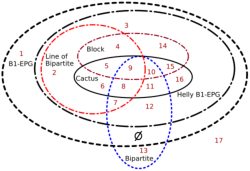
\includegraphics[width=8cm]{./img/diagram.pdf}
 \caption{Diagrama de algumas classes de grafos.}
\label{fig:diagram}
\end{figure}  
 


 \begin{figure}[htb]	
 
   \centering
  \begin{tabular}{  c c c c  c}
    %\centering
    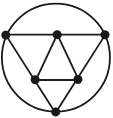
\includegraphics[width=2cm]{img/octaedroNoLabel.png} 
    & 
    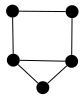
\includegraphics[width=1.5cm]{img/ex3.png} 
    & 
    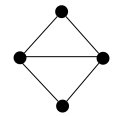
\includegraphics[width=2cm]{img/diamondNoLabel.png} 
    & 
    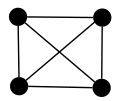
\includegraphics[width=1.5cm]{img/k4.png} 
    & 
    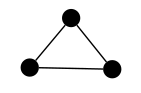
\includegraphics[width=2cm]{img/k3.png} 
    \\
    \footnotesize 
    (a)  \footnotesize Graph $E_1$. 
    & 
    \footnotesize (b) Graph $E_2$.
    & 
    \footnotesize (c) Graph $E_3$.
    & 
    \footnotesize (d) Graph $E_4$.
    & 
    \footnotesize (e) Graph $E_5$.
    \\%%Segunda linha
        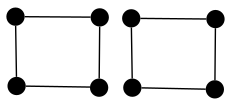
\includegraphics[width=2.5cm]{img/2c4.png} 
    & 
    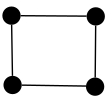
\includegraphics[width=1.5cm]{img/c4e.png} 
    & 
    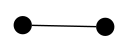
\includegraphics[width=1.8cm]{img/k2.png} 
    & 
    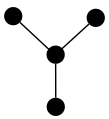
\includegraphics[width=1cm]{img/e10.png} 
    & 
    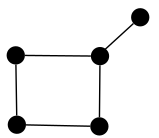
\includegraphics[width=1.8cm]{img/e11.png} 
    \\ %%Segundo Bloco legendas
    \footnotesize 
    (f)  \footnotesize Graph $E_7$. 
    & 
    \footnotesize (g) Graph $E_8$.
    & 
    \footnotesize (h) Graph $E_9$.
    & 
    \footnotesize (i) Graph $E_{10}$.
    & 
    \footnotesize (j) Graph $E_{11}$.
    %%Terceira linha de imagens
    \\%%Terceira linha
        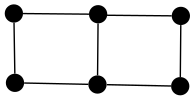
\includegraphics[width=2.5cm]{img/e12.png} 
    & 
    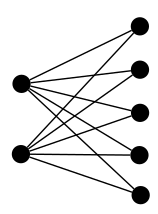
\includegraphics[width=2cm]{img/k25.png} 
    & 
    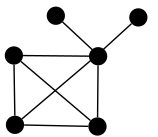
\includegraphics[width=2cm]{img/e14.png} 
    & 
    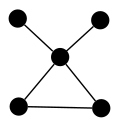
\includegraphics[width=1.8cm]{img/e15.png} 
    & 
    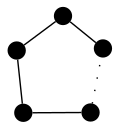
\includegraphics[width=1.8cm]{img/c2n+1.png} 
    \\ %%Terceiro Bloco legendas
    \footnotesize 
    (k)  \footnotesize Graph $E_{12}$. 
    & 
    \footnotesize (l) Graph $E_{13}$.
    & 
    \footnotesize (m) Graph  $E_{14}$.
    & 
    \footnotesize (n) Graph $E_{15}$.
    & 
    \footnotesize (o)  Graph $E_{16}$,  $C_{2n+1},n\geq2$.
    \\
    &&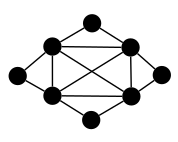
\includegraphics[width=2.5cm]{img/4sunNoLabel.png}&&
    \\
    &&\footnotesize (p)  Graph $E_{17}$.&&
    
    %\multicolumn{3}{c}{ \footnotesize (c) Another partial single bend representation of $H$ } \\
  \end{tabular}
 \caption{The set of instances for Venn Diagram of the graph classes of this paper.}
 %, see  more in~\cite{leveque2009characterizing,tondato2009grafos}
 \label{fig:exemplosDiagram}
\end{figure}  
 



















%  \begin{figure}[htb]	
 
%   \centering
%   \begin{tabular}{  c c c c  c}
%     %\centering
%     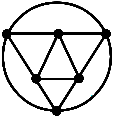
\includegraphics[width=1.7cm]{img/octaedro2.png} 
%     & 
%     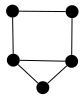
\includegraphics[width=1.5cm]{img/ex3.png} 
%     & 
%     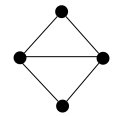
\includegraphics[width=2cm]{img/diamondNoLabel.png} 
%     & 
%     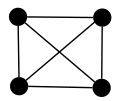
\includegraphics[width=1.5cm]{img/k4.png} 
%     & 
%     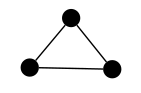
\includegraphics[width=2cm]{img/k3.png} 
%     \\
%     \footnotesize 
%     (a)  \footnotesize Grafo $E_1$. 
%     & 
%     \footnotesize (b) Grafo $E_2$.
%     & 
%     \footnotesize (c) Grafo $E_3$.
%     & 
%     \footnotesize (d) Grafo $E_4$.
%     & 
%     \footnotesize (e) Grafo $E_5$.
%     \\%%Segunda linha
%         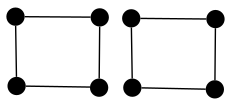
\includegraphics[width=2.5cm]{img/2c4.png} 
%     & 
%     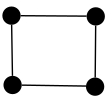
\includegraphics[width=1.5cm]{img/c4e.png} 
%     & 
%     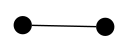
\includegraphics[width=1.8cm]{img/k2.png} 
%     & 
%     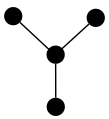
\includegraphics[width=1cm]{img/e10.png} 
%     & 
%     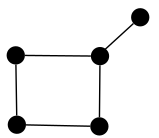
\includegraphics[width=1.8cm]{img/e11.png} 
%     \\ %%Segundo Bloco legendas
%     \footnotesize 
%     (f)  \footnotesize Grafo $E_7$. 
%     & 
%     \footnotesize (g) Grafo $E_8$.
%     & 
%     \footnotesize (h) Grafo $E_9$.
%     & 
%     \footnotesize (i) Grafo $E_{10}$.
%     & 
%     \footnotesize (j) Grafo $E_{11}$.
%     %%Terceira linha de imagens
%     \\%%Terceira linha
%         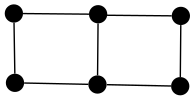
\includegraphics[width=2.5cm]{img/e12.png} 
%     & 
%     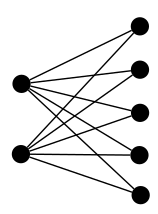
\includegraphics[width=2cm]{img/k25.png} 
%     & 
%     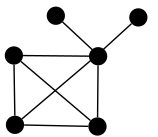
\includegraphics[width=2cm]{img/e14.png} 
%     & 
%     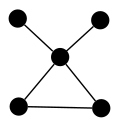
\includegraphics[width=1.8cm]{img/e15.png} 
%     & 
%     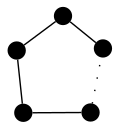
\includegraphics[width=1.8cm]{img/c2n+1.png} 
%     \\ %%Terceiro Bloco legendas
%     \footnotesize 
%     (k)  \footnotesize Grafo $E_{12}$. 
%     & 
%     \footnotesize (l) Grafo $E_{13}$.
%     & 
%     \footnotesize (m) Grafo  $E_{14}$.
%     & 
%     \footnotesize (n) Grafo $E_{15}$.
%     & 
%     \footnotesize (o)  Grafo $E_{16}$,  $C_{2n+1},n\geq2$.
%     \\
%     &&\includegraphics[width=2.5cm]{img/4sunNoLabel.png}&&
%     \\
%     &&\footnotesize (p)  Grafo $E_{17}$.&&
    
%     %\multicolumn{3}{c}{ \footnotesize (c) Another partial single bend representation of $H$ } \\
%   \end{tabular}
%  \caption{O conjunto de instâncias para o diagrama de Venn das classes de grafos estudadas até aqui.}
%  %, see  more in~\cite{leveque2009characterizing,tondato2009grafos}
%  \label{fig:exemplosDiagram}
% \end{figure}  
 

\section{Containment relationship among Chordal $B_1$-EPG, VPT and EPT graphs }


 Any graph that
admits a $B_1$-EPG representation  whose paths do not cover all the edges of a polygon of the grid (i.e.
the subjacent grid subgraph is a tree)  is also an EPT graph: the same representation is both $B_1$-EPG and $EPT$.
However, it is easily verifiable that the subjacent grid subgraph of any $B_1$-EPG representation of a cycle $C_n$ with $n\geq 5$ is not a tree,
%has a non chordal subjacent grid subgraph 
although $C_n$ is an  EPT graph.  Our long-rage goal is 
understanding the $B_1$-EPG graphs that are also EPT graphs. When can a $B_1$-EPG representation
be reorganized into an EPT representation?  In this section,
 we answer that question for Chordal $B_1$-EPG graphs, in fact we prove that every Chordal $B_1$-EPG graph is EPT. We
 made several unsuccessful attempts to prove this result by considering for a graph $G$, a $B_1$-EPG representation whose paths cover all the edges
 of some polygon on the grid, and trying  to show  that if none of the paths could be modified in order to avoid an edge of the polygon,
 then $G$ had some chordless  cycle (i.e. $G$ is not chordal). The surprise was that the only way we found to demonstrate our main Theorem \ref{teo:b1epgept} was through $VPT$ graphs.
 We will prove the following theorem.

\begin{theorem}\label{teo:chordalB1inVPT}
Chordal $B_1$-EPG $\subsetneq$ VPT. 
\end{theorem}

In~L{\'e}v{\^e}que et al. \cite{leveque2009characterizing} apud \cite{alcon2015characterizing},  VPT graphs were characterized by a family of minimal forbidden induced subgraphs,
the ones depicted in 
Figure~\ref{fig:16proibidos} plus the induced cycles $C_n$ for $n\geq 4$. Therefore, in order to prove
that Chordal $B_1$-EPG graphs are VPT is enough to show that none of the graphs in Figure~\ref{fig:16proibidos} 
is $B_1$-EPG. %The following lemmas are developed with that objective.   

First notice that in each one of the graphs $F_{1}, F_{2}, F_{3}, F_{4}$ and $F_{5}$ ( Figures~\ref{fig:16proibidos}(a), (b), (c), (d), (e), respectively), the neighborhood of the universal vertex (the one that is a bit bigger than the others, in the respective figures) contains an asteroidal triple. Therefore, by Lemma \ref{l:AT-free}, these graphs are not  $B_1$-EPG.

Now, in each one of the graphs $F_{11}, F_{12}, F_{13}, F_{14}$, $F_{15}$ and $F_{16}$  (Figures~\ref{fig:16proibidos}(k), (l), (m), (n), (o), (p), respectively), let $C$ be the maximal clique in bold. It is easy to check that, in all cases, the branch graph $B(G|C)$ contains an induced cycle $C_n$, for some $n\geq 4$, or an induced path $P_6$; thus, by Lemma \ref{l:branch},  graphs $F_{11}, F_{12}, F_{13}, F_{14}$, $F_{15}$ and $F_{16}$ are not $B_1$-EPG.



 % A \textit{satellite} of a clique $K$ is a vertex $v$ such that $B_v=N(v)\cap K$ is a 
%nonempty proper subset of $K$. The set $B_v$ is called the \textit{base} of $v$ and it is said \textit{minimal} if no other
%base of a satellite of $K$ is properly contained in $B_v$, see~\cite{alcon2010necessary}.

 %Let $I=[q_1,q_2]$ be the grid interval defined by the intersection $\displaystyle \cap_{v\in K}P_v$, where $K$
%is an edge-clique of a graph $G$. For any $v\in K$, by removing the interval $(q_1,q_2)$, the path $P_v$
%is split into two \textit{disjoint parts}: \textit{part 1}  containing $q_1$, and  \textit{part 2}  containing $q_2$.
%If $w$  is a satellite of $K$ adjacent to $v$, then
%$P_w\cap P_v$ is contained either in part 1 or in part 2 of $P_v$. We will say that $P_w$ intersects $P_v$
%on side 1 or on side 2 of $K$, respectively. Notice that if $w$  is also adjacent
%to another vertex $v'$ of $K$, then   $P_w$ intersects $P_v$ and $P_{v'}$ on
%a same side of $K$. It allow us to divide the satellites of $K$ into two \textit{disjoint
%groups}, the ones on  \textit{side 1} of $K$ and the ones on \textit{side 2}.

%%%%%%%%%%%%%%%%%%%%%%%%%%%
\begin{fac} \label{f:between}Let $e_{\ell}$, $e_m$ and $e_r$  be three distinct edges of a  one-bend path $P$, and assume that $e_m$ is between $e_{\ell}$ and $e_r$ on $P$. If $P_{\ell}$ and $P_r$ are one-bend paths such that: $P_{\ell}$ contains $e_{\ell}$, $P_r$ contains $e_r$, and  $P_{\ell}$ and $P_r$ intersect in at least one edge, then $P_{\ell}$ or $P_r$ contains $e_m$.
\end{fac}
%%%%%%%%%%%%%%%%%%%%%%%%%%%%%%
\begin{fac} \label{f:two points} Let  $e$ and $q$  be an edge and a  point  of a  one-bend path $P$, respectively. If a one-bend path $P'$ contains both $e$ and $q$, then $P'$ contains the whole segment of $P$ between $q$ and $e$.
\end{fac}

\begin{lema}\label{l:abclique}
Let $G$ be a graph whose vertex set  can be partitioned into a clique $K=\{a,b\}$ and an independent set $I=\{x,y,z\}$, such that each vertex of $K$ is adjacent to each vertex of $I$.
If in a given $B_1$-EPG representation of $G$, $P_a\cap P_y$ is between $P_a\cap P_x$ and $P_a\cap P_z$, then $\{a,b,y\}$ is an edge-clique, and
$P_a\cap P_y \subset P_b$. Even more, any vertex adjacent to $a$ and $y$, but not to $b$ (or to $b$ and $y$, but not to $a$) has to be adjacent to $x$ or to $z$.
\end{lema}

\begin{proof}
%%%%%%%%%%%%%%%%%%%%%%%%%%%%%%%
Assume in order to obtain a contradiction that $\{a,b,y\}$ is not an edge-clique. Then, by Lemma
\ref{lem:3cliquesNotClaw}, we can assume, w.l.o.g., that $\{a,b,x\}$ is an edge-clique.
It implies that there is an edge $e_{\ell}$ of $P_a \cap P_x$ covered by $P_b$. Since every  edge
of $P_a\cap P_z$ is covered  by $P_z$, $z$ and $b$ are adjacent, and $z$ and $y$ are non adjacent, we have by Fact \ref{f:between},
that every edge of $P_a\cap P_y$ is covered by $P_b$, which implies  that $\{a,b,y\}$ is an edge-clique, contrary to the assumption.

Thus, $\{a,b,y\}$ is an edge-clique. By Fact \ref{f:two points}, we have that the whole interval of $P_a$ between 
 $P_a \cap P_x$ and   $P_a \cap P_z$ is contained in $P_b$, and so, in particular, $P_a\cap P_y \subset P_b$. Observe that this
 implies that if $q$ is an end vertex of the interval $P_a \cap P_y$, and $e$ is the edge of $P_a$ incident on $q$ that do not belong to $P_y$, then 
$e$ belongs to $P_b$ or to $P_x$ or to $P_z$.
 
 Now, assume there exists a vertex $v$ adjacent to both $a$ and $y$ but not to $b$. Then, the clique $\{a,y,v\}$ has to be a claw-clique. Let $q$ be the center of the claw, notice that $q$ has to be an end vertex of the interval $P_a \cap P_y$.
 Since $v$ is not adjacent to $b$, it follows from the observation at the end of the paragraph above, that
 $v$ has to be adjacent to $x$ or to $z$.
\end{proof}

\begin{lema}\label{lem:F_6}
The graph $F_6$ on Figure~\ref{fig:16proibidos}(f) is not   $B_1$-EPG.
\end{lema}
\begin{proof} Let $K=\{1,2\}$ and $I=\{3,4,5\}$. If there exists a $B_1$-EPG representation of $F_6$,  by Lemma \ref{l:abclique},  because of the existence of the vertices $6$, $7$ and $8$, none of the vertices $3$, $4$ and $5$
may intersect $1$ between the remaining two, thus such a representation does not exist.
 \end{proof} 


\begin{lema}\label{lem:F_7}
The graph $F_7$ on Figure~\ref{fig:16proibidos}(g) is not   $B_1$-EPG.
\end{lema}
\begin{proof} Let $K=\{1,2\}$ and $I=\{4,5,6\}$. If there exists a $B_1$-EPG representation of $F_7$,  by Lemma \ref{l:abclique},  because of the existence of the vertices  $7$ and $8$, the vertex $6$ must intersect  vertex $1$ between $3$ and $4$. But considering $K'=\{1,3\}$, because of the existence of the vertices $5$ and $6$,  vertex $4$ must intersect vertex $1$ between $5$ and $6$. This contradiction implies that such a representation does not exist.
 \end{proof} 
 
 \begin{lema}\label{lem:F_8_9_10(8)}
The graphs $F_8$, $F_9$ and $F_{10}(8)$ on Figures~\ref{fig:16proibidos}(h), (i) and (j), respectively, are not   $B_1$-EPG.
\end{lema}
\begin{proof} Let $K=\{2,3\}$ and $I=\{1,5,7\}$. If there exists a $B_1$-EPG representation of any one of those graphs,  by Lemma \ref{l:abclique},  because of the existence of the vertices  $4$ and $8$, the vertex $1$ must intersect  vertex $2$ between $5$ and $7$. In addition, since $\{2,5,6\}$ is a clique, $6$ intersects $2$ in an edge of $P_5\cap P_2$ (edge-clique) or in an edge incident to $P_5\cap P_2$ (claw-clique). Analogously, because of the clique $\{2,7,6\}$,  $6$ intersects $2$ in an edge of $P_7\cap P_2$ (edge-clique) or in an edge incident to $P_7\cap P_2$ (claw-clique). In any case, it implies that $6$ intersects $2$ on two different edges, each one in a different side of $P_2 \cap P_1$, thus, by Fact \ref{f:two points}, $P_6$ contains the interval  $P_2 \cap P_1$, in contradiction with the fact that $1$ and $6$ are not adjacent.
  \end{proof} 



 \begin{figure}[htb]	
 
   \centering
  \begin{tabular}{  p{2.7cm} p{2.7cm} p{2.7cm} p{2.7cm} p{2.7cm} }
    %\centering
    \includegraphics[width=2.5cm]{img/f1.png} 
    & 
    \includegraphics[width=2.1cm]{img/f2.png} 
    & 
    \includegraphics[width=2.7cm]{img/f3.png} 
    & 
    \includegraphics[width=2.7cm]{img/f4.png} 
    & 
    \includegraphics[width=2.7cm]{img/f5.png} 
    \\
    \footnotesize 
    (a)  \footnotesize Graph $F_1$. 
    & 
    \footnotesize (b) Graph $F_2$.
    & 
    \footnotesize (c) Graph $F_3$.
    & 
    \footnotesize (d) Graph $F_4$.
    & 
    \footnotesize (e) Graph $F_5(n),n\geq7$.
    \\%%Segunda linha
        \includegraphics[width=2.5cm]{img/f6.png} 
    & 
    \includegraphics[width=2.7cm]{img/f7.png} 
    & 
    \includegraphics[width=3cm]{img/f8.png} 
    & 
    \includegraphics[width=3cm]{img/f9.png} 
    & 
    \includegraphics[width=3cm]{img/f10n2.png} 
    \\ %%Segundo Bloco legendas
    \footnotesize 
    (f)  \footnotesize Graph $F_6$. 
    & 
    \footnotesize (g) Graph $F_7$.
    & 
    \footnotesize (h) Graph $F_8$.
    & 
    \footnotesize (i) Graph $F_9$.
    & 
    \footnotesize (j) Graph $F_{10}(n)$, $n\geq  8$.
    %%Terceira linha de imagens
    \\%%Terceira linha
        \includegraphics[width=3cm]{img/f11.png} 
    & 
    \includegraphics[width=3cm]{img/f12.png} 
    & 
    \includegraphics[width=3cm]{img/f13.png} 
    & 
    \includegraphics[width=3cm]{img/f14.png} 
    & 
    \includegraphics[width=3cm]{img/f15.png} 
    \\ %%Terceiro Bloco legendas
    \footnotesize 
    (k)  \footnotesize  $F_{11}(4k),$ $k\geq2$. 
    & 
    \footnotesize (l)  $F_{12}(4k),$ $k\geq2$.
    & 
    \footnotesize (m)  $F_{13}(4k+1),$ $k\geq2$.
    & 
    \footnotesize (n)  $F_{14}(4k+1),$ $k\geq2$.
    & 
    \footnotesize (o)  $F_{15}(4k+2),$ $k\geq2$.
    
    \\ %Ultima linha Figuras
    
    && \includegraphics[width=3cm]{img/f16.png} &&
    
    \\%Ultima linha Legendas
    
    && \footnotesize (p)  $F_{16}(4k+3),$ $k\geq2$. &&
    
    %\multicolumn{3}{c}{ \footnotesize (c) Another partial single bend representation of $H$ } \\
  \end{tabular}
 \caption{The 16 Chordal induced subgraphs forbidden to VPT (the vertices in the cycle marked by bold edges form a clique).}
 %, see  more in~\cite{leveque2009characterizing,tondato2009grafos}
 \label{fig:16proibidos}
\end{figure}  
 

 \begin{figure}[htb]	
 \center%6.3
 \includegraphics[width=4cm]{./img/f10-8opc.png}
 \caption{Graph $F_{10}(8)'$ plus two optional edges.}
\label{fig:f10-8opc}
\end{figure}  
 



\begin{lema}\label{lem:f10}
The graph $F_{10}(n)$ is not a $B_1$-EPG graph. 
\end{lema}

\begin{proof}
The graph $F_{10}(n)$ presented in~\cite{alcon2015characterizing} (see Figure~\ref{fig:16proibidos}(j)) is a graph that has $n$ vertices and whose set $K$ is highlighted. This graph has $k=n-5$ vertices, where $k\geq 3, n\geq 8$. Note that each clique $F_{10}(n)[a, b, i]$, where $i \in K$ and  $2\leq i \leq k-1$, have the same  characteristic of the clique $F_{10}(8)[2, 3, 6]$  presented in Figure~\ref{fig:ktent}, that is in any single bend EPG representation these set of vertices are represented by edge-clique (see Lemma~\ref{lem:cliquesMaximais}).

We will prove that there exists a single bend  EPG representation for $F_{10}(n)$ if only if there exists a single bend  EPG representation for $F_{10}(n-1)$. Our induction  is on the set of vertices of $K$ and the paths that they represent.

%\input{includes/include-img/f10n.tex}

Given the graph $F_{10}(n)$, suppose there is a $B_1$-EPG representation $R$ for $F_{10}(n)$. By Lemma~\ref{lem:cliquesMaximais}, each clique $F_{10}(n)[a, b, i]$, where $i \in K$ and  $2\leq i \leq k-1$ is an edge-clique, then we need analyze two cases:

\begin{itemize}
    \item Case 1: Paths $\displaystyle P_{{k-1}}$ and $\displaystyle P_{{k}}$ are on same row/column.
    
    The interval between row/column where $ P_{{1}}$ intersects $ P_{{2}}$ through row/column that $ P_{{k-1}}$ intersects $ P_{{k}}$  necessarily has only paths of set $P_i \cup \{P_a,P_b\}$. No path $P_i$, $2 \leq i \leq k-1$, needs bend, except if $P_a$ or $P_b$ bend.
     As $R$ is a single bend EPG representation for $F_{10}(n)$ then when we remove the path $\displaystyle P_{{k}}$, we can preserve the intersection of $P_{{k}}$ in $P_{{k-1}}$ and now we have a representation $R'$ that is also a  single bend EPG representation for $F_{10}(n-1)$.
    
      \item Case 2: Paths $\displaystyle P_{{k-1}}$ and $\displaystyle P_{{k}}$ are on distinct rows/columns.
      
      Path $\displaystyle P_{{k}}$ is intersecting to $P_a, P_b, P_c$ and $\displaystyle P_{{k-1}}$. Path $P_c$ intersects $P_b$ and $\displaystyle P_{{k}}$. If $\displaystyle P_{b}$ bends then $P_b \cap P_c$ has that occur on this row/column. Or $\displaystyle P_{{k}}$ or $\displaystyle P_{{k-1}}$ has bend, and when we remove $\displaystyle P_{{k}}$ then $\displaystyle P_{{k-1}}$ has bend and now there exists $P_b \cap  P_c \cap $ $\displaystyle P_{{k-1}}$. If before removal $\displaystyle P_{{k}}$ the representation $R$ was a single bend EPG representation for $F_{10}(n)$ then now $R'$ remains a single bend EPG representation, but for $F_{10}(n-1)$.    
\end{itemize}

Yet by induction we know that there is a single bend EPG representation for $F_{10}(9)$ if only if there is a single bend EPG representation for $F_{10}(8)$, but by Corollary~\ref{coro:F108IsNotB1EPG} the graph $F_{10}(8)$ is not $B_1$-EPG, therefore we can conclude that $F_{10}(n)$ is not $B_1$-EPG.
%Thus $F_{10}$ is not a interval graph, so some path in an EPG representation of $F_{10}$ has at least one bend.
 \end{proof} 






%INSERIR DEFINICOES TRIPLA ASTEROIDAL, BRANCH GRAPH, Neighboor, numero cromatico
%The following definitions will be useful for complete our proof and to help us in the next demonstrations.

%The follow we compile results to conclude the proof.

%In the graphs $F_{1}, F_{2}, F_{3}, F_{4}$ and $F_{5}$ ( Figures~\ref{fig:16proibidos}(a), (b), (c), (d), (e), respectively), the neighborhood of the universal vertex contains an asteroidal triple, %thus these graphs are not $B_1$-EPG graphs.


%By Lemmas~\ref{lem:f6}, \ref{lem:f7},  Corollaries~\ref{coro:f8}, \ref{coro:f9}, \ref{coro:F108IsNotB1EPG} and Lemma~\ref{lem:f10}  from this paper, we know that the
%graphs $F_{6}, F_{7}, F_{8}, F_{9}$ and $F_{10}(n)$ ( Figures~\ref{fig:16proibidos}(f), (g), (h), (i), (j), respectively) are also not $B_1$-EPG graphs.


%In addition, by characterization of branch graph we state that none of the graphs $F_{11}(4k), F_{12}(4k), F_{13}(4k+1), F_{14}(4k+1)$, $F_{15}(4k+2)$ and $F_{16}(4k+3)$  %(Figures~\ref{fig:16proibidos}(k), (l), (m), (n), (o), (p), respectively) is a $B_1$-EPG graph.


We have proved that every minimal forbidden induced subgraph for VPT is also a minimal forbidden induced subgraph for $B_1$-EPG. So we can say that the class of Chordal $B_1$-EPG graphs is contained in the class of VPT graphs. Furthermore, there are graphs in VPT that do not belong to $B_1$-EPG, for instance the graph $4$-sun $S_4$ is not in $B_1$-EPG, see~\cite{golumbic2009}, but it has a VPT representation, see Figures~\ref{fig:exemplos}(a) and~\ref{fig:exemplos}(b). Thus, VPT graphs contain properly Chordal $B_1$-EPG graphs. This conclude the proof of Theorem~\ref{teo:chordalB1inVPT}.
 %\end{proof} 

\begin{figure}[htb]
  \centering
  \begin{tabular}{ c c c }
    \centering
    \includegraphics[width=5cm]{img/s4.png} & &
    \includegraphics[width=8cm]{img/s4eptRepresentation.png}
    \\
    \footnotesize \centering 
    (a)  \footnotesize Graph $S_4$. &&  \footnotesize (b) A VPT and EPT representation of $S_{4}$. \\

  \end{tabular}

 \caption{Graph $S_4$ and one of its possible VPT and EPT representations.}
 \label{fig:exemplos}
\end{figure} 


\begin{theorem}
(\cite{alcon2014recognizing}) Let $G$ be a VPT graph and $h\geq 4$. The graph $G$ belongs to $[h,2,1]-[h-1,2,1]$ if and only if max$_{C\in\mathcal{C}(G)}(\chi (B(G|C)))=h$. The reciprocal implication is also true for $h=3$.
\end{theorem}


%Grafo C_4 eh EPT mas nao eh Chordal
\begin{theorem}\label{teo:b1epgept}
Chordal $B_1$-EPG $\subsetneq$ EPT. 
\end{theorem}

\begin{proof}
Given $G$ be a  Chordal $B_1$-EPG graph and let  $\mathcal{C}$  be the set of cliques of $G$. By Theorem~\ref{teo:chordalB1inVPT}, we know that $G$ is VPT. By \cite{golumbic2009}, we know that if $G$ is $B_1$-EPG then $\chi (B(G|C))\leq 3$,  for all $C \in \mathcal{C}$. By a result given in ~\cite{alcon2014recognizing}, we can say that $G \in [3,2,1]$, and $[3,2,1] = VPT \cap EPT$, and $[3,2,1] = [3,2,2] = EPT$ $\cap$ Chordal~\cite{golumbic1985} then $G$ is a Chordal EPT graph. Therefore, Chordal $B_1$-EPG is contained in EPT. Moreover, the inclusion is proper because for example the graph $4$-sun $S_4$ is an EPT graph (see Figure~\ref{fig:exemplos}(b)) but it is not a $B_1$-EPG graph (see ~\cite{golumbic2009}).
 \end{proof} 



\section{Conclusion and Open Questions}

In this paper, we considered graphs of intersection of paths, in particular $B_1$-EPG, VPT and EPT graphs. We show that graphs $\{S_3, S_{3'},S_{3''},C_4\}$-free and others non-trivial subclasses of  $B_1$-EPG graphs have the Helly property, namely by instance Bipartite, Block, Cactus and Line of bipartite graphs. 
  
  In addition, combining the results of~\cite{alcon2014recognizing,Asinowski2009, golumbic2009} and some proves  presented in this paper, we demonstrate by  Theorems~\ref{teo:chordalB1inVPT} and~\ref{teo:b1epgept} that Chordal $B_1$-EPG graphs are simultaneously contained in the classes of VPT and EPT graphs.  
 
 
%If on the one hand some few graph classes are known to be properly contained in $B_1$-EPG, for instance the $L$-shaped paths graphs see~\cite{cameron2016edge},  and the recognition time for $B_1$-EPG graphs in general is $NP$-complete. On the other hand, in the course of this section we also present some subclasses of Helly-$B_1$ EPG for which the recognition problem is polynomial.

Asinowski and Ries present in~\cite{ries2009} some characterization for special cases of Split $B_1$-EPG graphs, when the stable set has size three or when the clique has size three. Observe that the graphs $F_2, F_{11}, F_{13}, F_{14}, F_{15}$, given in Figure~\ref{fig:16proibidos}, are Split but we used another strategy to prove that they are not $B_1$-EPG graphs. So one question is pertinent: Can we characterize Split graphs in general based in results of this paper? 

We would like to know the relationship of another graph subclasses of $B_1$-EPG with EPT and VPT graphs. If given an  input graph $G$ that is an instance of $B_1$-EPG  Weakly Chordal,  Distance-hereditary or any specific subclass, what is the relationship of $G$ with the class of paths in trees? For those same classes of graphs, what happens when we demand that the representations be Helly-$B_1$ EPG?

%%%%%%%%%%%%%%%%%%%%%%%%%%%%%%%%%%%%%%%%%
%%%%%%%%%%%%%%%%%%%%%%%%%%%%%%%%%%%%%%%%%
%%%%%%%%%%%%%%%%%%%%%%%%%%%%%%%%%%%%%%%%%
%%%%%%%%%%%%%%%%%%%%%%%%%%%%%%%%%%%%%%%%%
%%%%%%%%%%%%%%%%%%%%%%%%%%%%%%%%%%%%%%%%%
%%%%%%%%%%%%%%%%%%%%%%%%%%%%%%%%%%%%%%%%%
%%%%%%%%%%%%%%%%%%%%%%%%%%%%%%%%%%%%%%%%%
%%%%%%%%%%%%%%%%%%%%%%%%%%%%%%%%%%%%%%%%%
%%%%%%%%%%%%%%%%%%%%%%%%%%%%%%%%%%%%%%%%%
%%%%%%%%%%%%%%%%%%%%%%%%%%%%%%%%%%%%%%%%%
%%%%%%%%%%%%%%%%%%%%%%%%%%%%%%%%%%%%%%%%%
 
%\input{includes/include-img/diagramS3Free.tex}



% \section{Discussão Inicial}

% Modelos baseados em intersecção de caminhos podem ser considerados basicamente sob dois pontos de vista, o primeiro considera as intersecções em vértices e o segundo em arestas. Casos onde os caminhos são hospedados em uma árvore aparecem primeiro na literatura, veja por exemplo~\cite{gavril1978recognition, golumbic1985edge, golumbic1985}.  Representações usando caminhos sobre uma grade foram considerados mais tarde, ver~\cite{golumbic2009,golumbic2013, golumbic2013intersection}. A seguir detalharemos os modelos de intersecção que serão estudados neste capítulo. %More details on each intersection model will be given in the following text.

%  Seja $P$ uma família de caminhos sobre uma árvore hospedeira $T$. Dois tipos de grafos de intersecção do par  $<P,T>$ são definidos, denotaremos esses como grafos VPT e EPT.
% Os \textit{Grafos de Intersecção de Arestas} de $P$, EPT(P), possuem  vértices que correspondem aos membros de $P$, e dois vértices são  adjacentes em EPT(P) se e somente se os caminhos correspondentes em $P$ compartilham pelo menos uma aresta em $T$. Similarmente, os \textit{Grafos de Intersecção de Vértices} de $P$, VPT(P), possuem vértices que correspondem aos membros de  $P$, e dois vértices são adjacentes em VPT(P) se e somente se os caminhos correspondentes em  $P$ compartilham pelo menos um vértice em $T$. Em qualquer dos modelos considerados, sempre existe uma função de bijeção entre as intersecções dos caminhos e as adjacências dos vértices correspondentes. 


% Grafos VPT e EPT definem famílias incomparáveis de grafos. Entretanto, quando o grau máximo da árvore hospedeira é restrito a três, então a família dos grafos VPT coincide com a família dos grafos EPT~ \cite{golumbic1985edge% \cite{alcon2010necessary
% }. Também é conhecido que qualquer grafo Cordal EPT é também um grafo VPT (see~\cite{syslo1985triangulated}). Recordando também que outro resultado conhecido na literatura é o de que os grafos Cordais são os grafos de intersecção em vértices de subárvores de uma árvore, ver~\cite{gavril1974intersection}.


% \textit{Grafos de Intersecção de Caminhos sobre uma Grade} são chamados de \textit{grafos EPG}. 

% Em \cite{golumbic2009}, o autor provou que todos os grafos possuem uma representação EPG, e iniciou o estudo das subclasses definidas pela limitação do número de vezes que qualquer caminho utilizado na representação pode dobrar. Grafos admitindo uma representação onde caminhos possuem no máximo  $k$ mudanças de direção (dobras) foram chamados de grafos $B_k$-EPG. 
%  Em particular, quando os caminhos possuem no máximo uma dobra então temos os grafos \textit{ $B_1$-EPG}, também conhecidos como grafos EPG de  \textit{dobra simples}.

% Uma questão pertinente no contexto de grafos de intersecção de caminhos é como segue: dadas duas classes de de grafos de intersecção de caminhos,  a primeira cujo hospedeiro é uma árvore e a segunda cujo hospedeiro é uma grade, existe uma intersecção ou um relacionamento de continência entre essas classes? O que sabemos sobre isso?

% Nesse capítulo iremos explorar os grafos  $B_1$-EPG, em particular os grafos diamante-livre e os grafos Cordais. Trabalharemos principalmente sobre questões a respeito da relação de contenção entre as classes de grafos VPT, EPT e $B_1$-EPG.

% Uma coleção de conjuntos satisfaz a   \textit{propriedade Helly} quando toda subcoleção que é mutuamente intersectante possui pelo menos um elemento em comum. Quando essa propriedade é satisfeita pelo conjunto de vértices (ou arestas) dos caminhos utilizados na representação, então temos uma representação Helly. Grafos   $B_1$-EPG-Helly foram estudados em~\cite{bornstein2019}, que mostraram que todo grafo admite uma representação Helly e também que o problema de reconhecer grafos $B_1$-EPG-Helly é $NP$-completo.  

% É conhecido que nem todo grafo $B_1$-EPG admite uma representação  $B_1$-EPG-Helly. Estamos interessados em determinar os subgrafos que são grafos
% $B_1$-EPG porém não admitem uma representação  Helly $B_1$-EPG. Nesse capítulo, descrevemos estruturas que estarão presentes em qualquer desses subgrafos, além do mais, também apresentamos novas subclasses de grafos  $B_1$-EPG-Helly. Ademais, delimitamos novas subclasses $B_1$-EPG-Helly e damos alguns  conjuntos de subgrafos que delimitam subfamílias Helly.
% \section{Definições e Resultados Técnicos}

% O \textit{conjunto de vértices} e o \textit{conjunto de arestas} de um grafo  $G$ são denotados por $V(G)$ e $E(G)$, respectivamente.  Dado um vértice  $v\in V(G)$,  $N(v)$ e $N[v]$ representam a   \textit{vizinhança} aberta e fechada de  $v$ em $G$, respectivamente. 
% Para um subconjunto  $S \subseteq V(G)$,  $G[S]$ é o subgrafo de $G$ induzido por $S$.
%  Se $\mathcal{F}$ é uma família qualquer de grafos, dizemos que $G$ é  \textit{$\mathcal{F}$-livre} se $G$ não possui subgrafo induzido isomorfo a um membro de $\mathcal{F}$.
%  Um \textit{ciclo},  denotado por $C_n$, é uma sequência de vértices distintos  $v_1, \dots , v_n, v_1$  onde $v_i \neq v_j$ for $i \neq j$ e $(v_i, v_i + 1) \in E(G)$, tal que $n \geq 3$. Uma \textit{corda} é uma aresta que está entre dois vértices não-consecutivos em uma sequência de vértices de um ciclo. Um \textit{ciclo induzido}  ou \textit{ciclo sem corda} é um ciclo que não possui corda, nesse capítulo todo ciclo induzido será chamado simplesmente de  \textit{ciclo}. Um grafo  $G$ formado por um ciclo induzido $H$ mais um único vértice universal  $v$ conectado a todos vértices de $H$ é chamado  \textit{grafo roda}. Se o grafo roda possui $n$ vértices, ele é denotado por $n$-roda. 

% O grafo $k$\textit{-sol} $S_k$, $k \geq 3$, consiste de 
% $2k$ vértices, um conjunto independente $X = \{x_1, \dots, x_k\}$ e uma clique $Y = \{y_1, \dots, y_k\}$, e um conjunto de arestas $E_1 \cup E_2$, onde $E_ 1=\{ (x_1,y_1); (y_1, x_2); (x_2, y_2); (y_2, x_3); \dots , (x_k, y_k); (y_k, x_1) \}$ forma o ciclo externo e $E_2= \{(y_i, y_j) |i\neq j\}$ forma uma clique interna.

% Um grafo é $ B_k$-EPG se ele admite uma representação EPG em que cada caminho possui no máximo $k$ dobras. Quando $ k = 1 $ dizemos que essa é uma representação \emph{ EPG de dobra simples} ou simplesmente uma representação  $B_1$-EPG. 
% Uma \textit{clique} é um conjunto de vértices mutuamente adjacentes, enquanto
% um \textit{conjunto independente} é um conjunto de vértices não mutuamente adjacentes entre si.
%  Dada uma representação EPG de um grafo  $G$, identificaremos cada vértice  $v$ de $G$ com o correspondente caminho  $P_{v}$ da grade, utilizado na representação. Adequadamente, por exemplo, diremos que um vértices de  $G$ cobre ou contem alguma aresta da grade (significando que o correspondente caminho faz isso), ou que o conjunto de caminhos da representação induz um subgrafo de $G$ (significando que o correspondente conjunto de vértices faz isso, na verdade). 

% Em uma representação $B_1$-EPG, uma clique $K$ é dita ser uma \textit{clique-aresta} se todos os vértices de $K$ compartilham pelo menos uma aresta comum da grade (ver Figura~\ref{fig:cliquesRepresentation}(a)).
%  Uma \textit{garra da grade} é um conjunto de três arestas da grade, incidentes no mesmo ponto da grade, que é chamado o \textit{centro da garra}. As duas arestas da garra que tem a mesma direção formam a  \textit{ base da garra}. Se $K$ não é uma clique-aresta, então existe uma garra da grade   (e somente uma) tal que os vértices de  $K$ são aqueles que contem exatamente duas das três arestas dessa garra; tal clique é chamada de   \textit{clique-garra} \cite{golumbic2009} (ver Figura~\ref{fig:cliquesRepresentation}(b)).

    
% 
\begin{figure}[h]
  \centering
  \begin{tabular}{  p{4.5cm} p{0.7cm} p{4cm} }
    %\centering
    \includegraphics[width=4.5cm]{img/edge-clique.png} & &
    \includegraphics[width=3.5cm]{img/claw-clique.png}%b1EpgTransparenteGrade2
    \\
    \footnotesize %\centering 
    (a)  \footnotesize Representation of a clique as edge-clique. && \footnotesize (b) Representation  of a clique as claw-clique.\\
  \end{tabular}

 \caption{Examples of clique representations.} \label{fig:cliquesRepresentation}
\end{figure}


















% \begin{figure}[h]
%   \centering
%   \begin{tabular}{  p{4cm} p{0.7cm} p{4cm} }
%     %\centering
%     \includegraphics[width=4.5cm]{img/edge-clique.png} & &
%     \includegraphics[width=3.5cm]{img/claw-clique.png}%b1EpgTransparenteGrade2
%     \\
%     \footnotesize %\centering 
%     (a)  \footnotesize Representação de uma  clique como clique-aresta. && \footnotesize (b) Representação de uma  clique como clique-garra.\\
%   \end{tabular}

%  \caption{Exemplos de representações de clique.} \label{fig:cliquesRepresentation}
% \end{figure}    

% Note que se três vértices induzem uma clique-garra, então exatamente dois deles dobram no centro da garra correspondente na grade, e o terceiro contem a base da garra.
% Além disso, qualquer outro vértice adjacente aos três deve conter duas das arestas dessa garra, então o seguinte lema é válido.

% \begin{lema}\label{lem:cliquesMaximais}
% Se três vértices estão juntos em mais que uma  clique maximal do grafo $G$, então em qualquer representação $B_1$-EPG de $G$ esses três vértices não formam uma  clique-garra.
% \end{lema}

% \begin{figure}[ht]
  \centering
  \begin{tabular}{  p{5cm} p{0.7cm} p{5cm} }
    %\centering
    \includegraphics[width=3.5cm]{img/lemaClaw2Maximais} & &
    \includegraphics[width=5.5cm]{img/claw2}
    \\
    \footnotesize %\centering 
    (a)  \footnotesize Examplo de duas cliques maximais compartilhando vértices. && \footnotesize (b) Representação de uma clique-garra na grade.\\
  \end{tabular}

 \caption{Vértices representados por uma garra  estão presentes em uma única clique maximal.} \label{fig:lemaClaw2Maximais}
\end{figure}

% Em Asinowski et al. \cite{ries2009} foi provado o seguinte lema para grafos $C_4$-livre.

% \begin{lema} \cite{ries2009} \label{lem:lemaBRies2009}
% Seja $G$ um grafo $B_1$-EPG. Se $G$ é $C_4$-livre, então existe uma representação $B_1$-EPG de $G$ tal que toda clique-garra maximal $K$ é representada sobre uma  garra da grade cuja base é coberta unicamente por vértices de $K$.
% \end{lema}


% Temos obtido o seguinte resultado, similar para grafos diamante-livre. Um \textit{diamante} é um grafo  $G$ com conjunto de vértices  $V(G) = \{a, b, c, d\}$ e conjunto de arestas $E(G)=\{ab, ac,bc, bd,cd\}$ (ver Figura~\ref{fig:diamond}). %A graph is diamante-livre if it does not contain a diamante as induced subgraph.

%  \begin{figure}[htb]	
 \center%6.3
 \includegraphics[width=2.2cm]{./img/diamond.png}
 \caption{Diamond graph.}
\label{fig:diamond}
\end{figure}  
 


% \begin{lema}\label{lem:b1epgDiamondFree}
% Seja $G$ um grafo $B_1$-EPG. Se $G$ é diamante-livre, então em qualquer representação $B_1$-EPG de $G$,  toda  clique-garra maximal $K$ é representada sobre uma garra da grade cujas arestas são cobertas somente por  vértices de $K$.
% \end{lema}

% \begin{proof}Seja $K$ uma  clique maximal que é uma clique-garra em uma dada representação $B_1$-EPG de $G$. Então existem três  vértices de $K$ que induzem uma  clique-garra $K'$ sobre a mesma garra da grade que $K$. Assuma, de forma a derivar uma contradição, que um vértice $v\notin K$ cobre alguma aresta da garra. Claramente, $v$ deve cobrir somente uma das arestas. Portanto $v$ e os vértices de $K'$ induzem um  diamante, uma contradição.
% \end{proof}


% % \begin{defi} \label{defi:tortasFrame}

% Seja $ Q $ uma grade e sejam $ (a_1, b),$ $(a_2, b),$ $(a_3, b),$ $(a_4, b)$ uma $4$-estrela centrada em $b$ como ilustrado na Figura~\ref{fig:piesInGrid}(a). Seja $ \mathcal{P} = \{P_1, \dots , P_4\}$ uma coleção de quatro caminhos cada um contendo um diferente par de arestas da $4$-estrela.
% %exactly two edges of the $4$-estrela:
% Seguindo \cite{golumbic2009}, dizemos que esses quatro caminhos formam:

% \begin{itemize}
% \item uma \emph{torta verdadeira}  quando cada um possui uma dobra em  $b$, Figura~\ref{fig:piesInGrid}(b); e
% \item uma \emph {torta falsa} quando exatamente dois dos caminhos dobram em  $b$ e eles não compartilham aresta da $4$-estrela, Figura~\ref{fig:piesInGrid}(c). %contain bends, while the remaining two do not share an edge. 

% \begin{figure}[htb]
  \centering
%segundo bloco de figuras
  \begin{tabular}{c c c c c }
    \includegraphics[width=3.5cm]{img/disposicaoTortaGrid3.pdf}    
    & &\includegraphics[width=3.5cm]{img/truePieGrid} 
    & &
 \includegraphics[width=3.5cm]{img/falsePieGrid} \\%[\abovecaptionskip]
    {\footnotesize (a) 4-estrela em uma grade.}  & &  {\footnotesize (b) Torta verdadeira.} & & {\footnotesize (c) Torta falsa.} 
  \end{tabular}
  \caption{Representação $B_{1}$-EPG do ciclo induzido de tamanho  4 como tortas, com ênfase no centro $b$.}\label{fig:piesInGrid}
\end{figure} 

% %\vspace{-0.5cm}
% \end{itemize}
% % \end{defi}

% Claramente se quatro caminhos de uma representação $B_1$-EPG de $G$ formam uma torta, então os vértices correspondentes induzem um $4$-ciclo em $G$. % The converse implication is also true (see~\cite{golumbic2009}). 
% O seguinte resultado pode ser facilmente provado. Dizemos que um conjunto de caminhos forma uma garra quando cada par de arestas da  garra está coberto por algum dos caminhos.

% \begin{lema}\label{lem:twogarraNotSameCenterInCordal}
% Em qualquer representação $B_1$-EPG de um grafo $G$, um conjunto de caminhos formando duas diferentes garras centradas no mesmo ponto da grade contem quatro caminhos formando também uma torta verdadeira ou uma torta falsa. Portanto, em qualquer representação $B_1$-EPG de um grafo Cordal $G$, não existem duas  clique-garras maximal  $G$ centradas no mesmo ponto da  grade.
% \end{lema}

% \begin{lema}\label{lem:3cliquesNotgarra}
% Seja $G$ um grafo cujo conjunto de vértice pode ser particionado em uma clique não trivial $K$ e um conjunto independente $I=\{w_1,w_2,w_3\}$, tal que cada vértice de $K$  é adjacente a cada vértice de $I$. Então, em qualquer representação $B_1$-EPG de $G$,  pelo menos uma das cliques  $K_i = K \cup \{w_i\}$, com $1 \leq i \leq 3$,  é uma clique-aresta. 
% \end{lema}

% \begin{proof}
% Assuma, de forma a derivar uma contradição, que as três cliques são cliques-garra. Pelo Lema~\ref{lem:twogarraNotSameCenterInCordal}, eles possuem diferentes centros. Digamos que os centros dessas cliques-garra sejam os pontos $q_1, q_2, q_3$ da grade, respectivamente. Uma vez que pelo menos dois caminhos possuem uma dobra no centro de uma garra, para cada $i\in\{1,2,3\}$,   deve existir um vértice
%   $v_i$ de $K$ tal que o caminho correspondente $P_{v_i}$ dobra no ponto $q_i$ da grade.  Note que cada um dos três caminhos $P_{v_i}$ devem conter os três pontos da grade,  $q_1$, $q_2$ e $q_3$. Para provar que isso não é possível, consideraremos, sem perda de generalidade, dois casos.
%   No primeiro,  $q_1$ está entre $q_2$ e $q_3$ em $P_{v_1}$. Então, $P_{v_3}$ não pode dobrar em $q_3$ e conter $q_1$ e $q_2$.   No segundo caso,
%   $q_2$ está entre $q_1$ e $q_3$ em $P_{v_1}$. Dessa forma, $P_{v_2}$ não pode dobrar em  $q_2$ e conter $q_1$ e $q_3$; assim a prova está completa.
% \end{proof}

% Três vértices $u, v, w$ de um grafo $G$ formam uma \textit{ tripla asteroidal } (AT) de  $G$ se para todo par deles existe um caminho conectando esses dois  vértices e tal que o caminho evita a vizinhança do vértice remanescente~\cite{Asinowski2009}. Um grafo sem uma tripla asteroidal é chamado \textit{AT-livre}. 

% \begin{lema}
% [\cite{ries2009}] \label{l:AT-livre} Seja $v$ qualquer vértice de um grafo $B_1$-EPG  $G$. Então $G[N(v)]$ é AT-livre.
% \end{lema}

% Seja $C$ qualquer subconjunto dos vértices de um grafo $G$. O \textit{grafo branch} $B(G|C)$, ver~\cite{golumbic2009}, de $G$ sobre $C$ possui um conjunto de vértices, $V(B)$, consistindo de todos os vértices de $G$ que não pertencem a $C$ mas são adjacentes a algum membro de  $C$, i.e. $V(B) = N(C) - C$. As adjacência em $B(G|C)$ são definidas como segue: unimos dois vértices $x$ e $y$ por uma aresta em  $E(B)$ se e somente se em $G$ ocorre:
% \begin{enumerate}
%     \item  $x$ e $y$ são não adjacentes;
%     \item $x$ e $y$ possuem um vizinho comum $u \in C$;
%     \item os conjuntos $N(x) \cap C$ e $N(y) \cap C$ são incomparáveis, i.e. existem vizinhos privados $w, z \in C$ tal que $w$ é adjacente a $x$ mas não a $y$, e $z$ é adjacente a $y$ mas não é adjacente a $x$; dizemos que $x$ e $y$ são incomparáveis por vizinhança.
% \end{enumerate}

% Um grafo $G$ é \textit{k-colorável} se seus vértices podem ser coloridos com no máximo $k$ cores de forma que vértices adjacentes não compartilhem da mesma cor.

% \begin{lema}[~\cite{golumbic2009}] \label{l:branch} Seja $C$ qualquer clique maximal de um grafo $B_1$-EPG $G$. Então, o grafo branch $B(G|C)$ é $\{P_6, \, C_n \hbox{ para }  n\geq 4\}$-livre.
% \end{lema}





% \section{Subclasses de Grafos $B_1$-EPG-Helly}

% Nessa seção, delimitaremos algumas subclasses de grafos  $B_1$-EPG que admitem uma representação $B_1$-EPG-Helly. É conhecido que as classes de grafos $B_1$-EPG e $B_1$-EPG-Helly são classes hereditárias, assim elas podem ser reconhecidas por um conjunto de estruturas proibidas. 
% Em ambos os casos, encontrar a lista de subgrafos induzidos proibidos que delimita essas classes é um desafiante problema em aberto. 
% Dando um passo em direção a solucionar esses problemas, essa seção apresenta algumas estruturas onde pelo menos uma delas estará necessariamente presente em qualquer grafo $B_1$-EPG que não admita uma representação $B_1$-EPG-Helly. Além disso, mostramos que as já bem conhecidas famílias de grafos Bloco, Cactus e Linha de Bipartido estão totalmente contidas na classe dos grafos  $B_1$-EPG-Helly.


% Sejam $S_{3}, S_{3'}, S_{3''}$ e $ C_{4}$ os grafos ilustrados na  Figura~\ref{fig:proibidos}. 


% \begin{theorem}
% \label{lem:CordalDiamondFree}
% Seja $G$ um grafo $B_1$-EPG. Se $G$ é  $\{S_{3}, S_{3'}, S_{3''}, C_{4}\}$-livre então $G$ é um grafo $B_1$-EPG-Helly.
% \end{theorem}

% \begin{proof}
% Se $G$ não é um grafo $B_1$-EPG-Helly, então em qualquer representação $B_1$-EPG de $G$, existe pelo menos uma  clique que é representada como clique-garra e não como  clique-aresta. Considere qualquer representação $B_1$-EPG  de $G$  e seja $K$ uma clique maximal  que é representada como uma clique-garra. Assuma, sem perda de generalidade,  que $K$ está sobre uma garra da grade com base $[x_0, x_2]\times\{y_0\}$ e centro $C = (x_1, y_0)$. Denote por   $\mathcal{P}_K$ o conjunto de caminhos correspondendo aos  vértices de $K$. Pelo Lema~\ref{lem:lemaBRies2009}, os segmentos $[x_0, x_2]\times\{y_0\}$ da grade são cobertos somente por vértices de $K$. % because $G$ is $C_4$-livre


%  Para todo ${\displaystyle \lrcorner}$-caminho %$P_v \in \mathcal{P}_K$ 
%  (resp. ${\displaystyle \llcorner}$-caminho 
% % $P_{v'} \in \mathcal{P}_K$
%  ) pertencendo a $\mathcal{P}_K$, fazemos o seguinte: se o caminho não intersecta nenhum caminho $P_t \notin\mathcal{P}_K$ sobre a  coluna $x_1$, então deletamos seus segmento vertical e adicionamos o segmento  $[x_1, x_2]\times\{y_0\}$ (resp. $[x_0, x_1]\times\{y_0\}$) à grade. Se depois dessa transformação não existe mais  ${\displaystyle \lrcorner}$-caminhos (resp. ${\displaystyle \llcorner}$-caminhos) em $\mathcal{P}_K$, então temos efetuado a correção corretamente e obtemos uma clique-aresta. Assim podemos assumir que todo  ${\displaystyle \lrcorner}$-caminho   e todo ${\displaystyle \llcorner}$-caminho  em $ \mathcal{P}_K$ intersecta algum caminho $P_t \notin \mathcal{P}_K$ sobre a  coluna $x_1$ (note que podemos assumir que este é o mesmo  caminho $P_t$ para todos os vértices vértices). 
 
%  Agora, se nenhum dos  ${\displaystyle \lrcorner}$-caminhos pertencendo a $\mathcal{P}_K$ intersecta um caminho que não está em  $ \mathcal{P}_K$ sobre a linha $y_0$, então podemos substituir a parte  horizontal desses caminhos pelo segmento $[x_1,x_2]\times \{y_0\}$, obtendo uma representação por clique-aresta da clique $K$. Assim, podemos assumir que existe pelo menos um  ${\displaystyle \lrcorner}$-caminho $P_{v} \in \mathcal{P}_K$ intersectando algum caminho  $P_{t'} \notin \mathcal{P}_K$ sobre a linha $y_0$. Analogamente, existe no mínimo um  ${\displaystyle \llcorner}$-caminho $P_{v'} \in \mathcal{P}_K$ intersectando algum caminho $P_{t''} \notin K$ sobre a linha $y_0$, como ilustrado na Figura~\ref{fig:clawGrid}. Note que o vértice $t'$ não pode ser adjacente a qualquer dos vértices $t$, $v'$ ou $t''$; e, além disso, o vértice $t''$ não pode ser adjacente a $t$,  ou $v$.
 
%  Finalmente,   uma vez que $K$ é clique-garra,  existe um caminho $P_u \in \mathcal{P}_K$ cobrindo a base da garra. Dependendo das adjacências possíveis entre  $u$ e $t'$ ou   $t''$, um dos grafos  $S_{3}$, $S_{3'}$ ou $S_{3''}$ é obtido.
% \end{proof}

% 

\begin{figure}[h]
  \centering
  \begin{tabular}{  c p{0.7cm} c}
    %\centering
    \includegraphics[width=5.5cm]{img/clawGrid} & &
    \includegraphics[width=3.5cm]{img/clawInduced.png}
    \\
    \footnotesize %\centering 
    (a)  \footnotesize Claw with paths. && \footnotesize (b) Subgraph induced by paths.\\
  \end{tabular}

 \caption{Reconstruction of the intersection model.}
 \label{fig:clawGrid}
\end{figure} 

 


% \begin{figure}[h]
%   \centering
%   \begin{tabular}{  c p{0.7cm} c}
%     %\centering
%     \includegraphics[width=5.5cm]{img/clawGrid} & &
%     \includegraphics[width=3.5cm]{img/clawInduced.png}
%     \\
%     \footnotesize %\centering 
%     (a)  \footnotesize Clique-garra com caminhos adicionais. && \footnotesize (b) Subgrafo induzido pelos caminhos.\\
%   \end{tabular}

%  \caption{Reconstrução do modelo de intersecção.}
%  \label{fig:clawGrid}
% \end{figure} 

 



% Note  que qualquer grafo toro-livre é $\{S_{3}, S_{3'}, S_{3''}\}$-livre, assim nosso resultado anterior implica no Lema 5 de~\cite{ries2009}.

% 
\begin{figure}[h]
  \centering
  \begin{tabular}{  c p{0.7cm} c }
    \centering
    \includegraphics[width=4cm]{img/s3.png} & &
    \includegraphics[width=4cm]{img/s3-1.png}
    \\
    \footnotesize \centering 
    (a)  \footnotesize Grafo $S_3$. &&  \footnotesize (b) Grafo $S_{3'}$. \\
    
    %---------------------
      \centering 
      \includegraphics[width=4cm]{img/s3-2.png} & &
    \includegraphics[width=3cm]{img/c4.png}
    \\
    \footnotesize \centering 
    (c)  \footnotesize Grafo $S_{3''}$. && \footnotesize (b) Grafo $C_{4}$.\\
  \end{tabular}

 \caption{Grafos do enunciado do  Teorema~\ref{lem:chordalDiamondFree}.}
 \label{fig:proibidos}
\end{figure} 



% %--------------------------


% O próximo teorema possui como consequência a identificação de algumas classes de grafos onde a existência de uma  representação $B_1$-EPG implica na existência de uma representação  $B_1$-EPG-Helly.


% \begin{theorem} \label{lem:b1DiamondFree}
%  Se $G$ é um grafo $B_1$-EPG e diamante-livre então $G$ é um grafo $B_1$-EPG-Helly.
%  \end{theorem}

% \begin{proof}
% Se $G$ não é um grafo $B_1$-EPG-Helly, então em cada representação $B_1$-EPG de $G$, existe pelo menos uma clique que é representada como clique-garra e não como clique-aresta.  Considere qualquer representação $B_1$-EPG de $G$  e seja $K$ uma clique maximal que é representada como uma clique-garra. Assuma, sem perda de generalidade, que $K$ está sobre uma garra da grade com base $[x_0, x_2]\times\{y_0\}$ e centro $C = (x_1, y_0)$. Denote por  $\mathcal{P}_K$ o conjunto de caminhos correspondendo aos vértices de $K$. 
%  Pelo Lema~\ref{lem:b1epgDiamondFree},  %(see~\cite{ries2009})
% %no path $P_w$ for $w\notin K$ covers 
% o segmento da grade $[x_0, x_2]\times\{y_0\}$ é coberto somente por vértices de $K$. % because $G$ is $C_4$-livre
%  Para todo  ${\displaystyle \lrcorner}$-caminho %$P_v \in \mathcal{P}_K$ 
%  (resp. ${\displaystyle \llcorner}$-caminho 
% % $P_{v'} \in \mathcal{P}_K$
%  ) pertencente a  $\mathcal{P}_K$, fazemos o seguinte: se %$P_v$ (resp. $P_{v'}$)
%  o caminho não intersecta qualquer caminho $P_t \notin\mathcal{P}_K$ sobre a coluna $x_1$, então deletamos seu segmento vertical e adicionamos na grade o segmento $[x_1, x_2]\times\{y_0\}$ (resp. $[x_0, x_1]\times\{y_0\}$). Se depois dessa transformação não existir mais nenhum ${\displaystyle \lrcorner}$-caminhos (resp. ${\displaystyle \llcorner}$-caminhos) em $\mathcal{P}_K$, então terminamos, uma vez que temos obtido uma clique-aresta. Agora, podemos assumir que todo  ${\displaystyle \lrcorner}$-caminho   e todo ${\displaystyle \llcorner}$-caminho em $ \mathcal{P}_K$ intersecta algum caminho $P_t \notin \mathcal{P}_K$   sobre a coluna $x_1$ (note que podemos assumir que é o mesmo caminho $P_t$ para todos os vértices). Uma vez que $K$ é clique-garra, existe um caminho $P_u \in \mathcal{P}_K$ cobrindo a base da garra. Assim, $G[v, v', u, t]$ induz um diamante, uma contradição.
% \end{proof}  

% Um \textit{conjunto independente} de vértices é um conjunto de vértices não dois a dois adjacentes.
% Um grafo $G$ é dito ser \textit{Bipartido} se seu conjunto de vértices pode ser particionado em dois conjuntos independentes distintos.
%  Existem grafos Bipartidos que não são grafos $B_1$-EPG, por exemplo o grafo $K_{2,5}$ e $K_{3,3}$ (veja explicação em~\cite{cohen2014}). Claramente, uma vez que grafos Bipartidos são triângulo-livre, qualquer representação $B_1$-EPG de um grafo Bipartite é também uma representação $B_1$-EPG-Helly.
%  Um resultado similar (mas um pouco mais fraco) é obtido como corolário do teorema anterior.


% \begin{corollary}
% Se $G$ é um grafo Bipartido $B_1$-EPG então $G$ é um grafo $B_1$-EPG-Helly.
% \end{corollary}

% \begin{proof}
% Os grafos Bipartidos são diamante-livre, assim pelo Teorema~\ref{lem:b1DiamondFree} esses grafos são grafos $B_1$-EPG-Helly.
% \end{proof}

% Um \textit{grafo Bloco } ou \textit{grafo Árvore Clique} é um tipo de grafo em que toda componente biconexa (bloco) é uma clique.

% \begin{corollary}\label{lem:cdf}
%  Grafos Bloco são $B_1$-EPG-Helly.
% \end{corollary}

% \begin{proof}
% Grafos Bloco são conhecidos por corresponderem exatamente à classe de grafos Cordal diamante-livre, assim pelo Teorema 19 de \cite{ries2009}, todos grafos Bloco são grafos  $B_1$-EPG. Segue do Teorema~\ref{lem:b1DiamondFree} que todos grafos Bloco estão na classe de grafos $B_1$-EPG-Helly. 
% \end{proof} 

% Um \textit{grafo Cactus} (algumas vezes chamado também de Árvore Cactus) é um grafo conexo em que quaisquer dois ciclos possuem no máximo um vértice em comum. Equivalentemente, ele é um grafo conexo em que toda aresta pertence a no máximo um ciclo, ou (para um cactus não trivial) em que cada bloco (subgrafo maximal sem vértice de corte) é uma aresta ou um ciclo. A família de grafos em que cada componente é um Cactus é fechada sob operações menores de grafos. Essa família de grafos pode ser caracterizada por um único subgrafo proibido menor, o grafo diamante.
 
% \begin{corollary}
% Grafos Cactus são  $B_1$-EPG-Helly.
% \end{corollary}
% \begin{proof}
% Em~\cite{cela2019monotonic} foi provado que todo grafo Cactus graph é um grafo  $B_1$-EPG monotônico 
% (existe uma representação $B_1$-EPG onde todos os caminhos são ascendentes em linhas e colunas). 
% Assim, grafos Cactus são grafos $B_1$-EPG. 

% Uma vez que Cactus são diamante-livre, pelo Teorema~\ref{lem:b1DiamondFree}, a prova segue verdadeira.
% \end{proof}

% Dado um grafo $G$, seu \textit{grafo Linha} $L(G)$ é um grafo tal que cada vértice de $L(G)$ representa uma aresta de  $G$ e dois  vértices de $L(G)$ são adjacentes se e somente se suas arestas correspondentes compartilham um vértice comum (i.e. elas ``são incidentes'' em um mesmo vértice) em $G$.  
% Um grafo $G$ é um \textit{grafo Linha de um grafo Bipartido} (ou simplesmente \textit{Linha de Bipartido}) se e somente se ele não contem  garra, nem ciclo ímpar, e nem diamante como subgrafo induzido, \cite{harary1974line}.



% \begin{corollary}\label{coro:lineOfBipartido}
%  Grafos Linha de Bipartido são $B_1$-EPG-Helly. 
% \end{corollary}

% \begin{proof}
% Grafos Linha de Bipartido foram provados ser $B_1$-EPG in~\cite{golumbic2018edge}. Uma vez que eles são diamante-livre, a prova segue diretamente pelo Teorema~\ref{lem:b1DiamondFree}.
% \end{proof}

% O diagrama da Figura~\ref{fig:diagram}
% ilustra o relacionamento de continência entre as classes de grafos estudadas até agora neste trabalho.  
% Listamos na Figura~\ref{fig:exemplosDiagram} exemplos de grafos em cada região numerada do diagrama. Os números de cada item abaixo correspondem às respectivas regiões com mesmo número do diagrama ilustrado na Figura~\ref{fig:diagram}.

% %This numbers correspond with the respective number item and in some cases we make a brief explanation.

%  \begin{figure}[htb]	
 \center%6.3
 \includegraphics[width=8cm]{./img/diagram.pdf}
 \caption{Diagrama de algumas classes de grafos.}
\label{fig:diagram}
\end{figure}  
 

% \begin{enumerate}[label=(\arabic*)]
%     \item Grafos $B_1$-EPG  - $B_1$-EPG-Helly, ilustrado na Figura~\ref{fig:exemplosDiagram}(a), grafo $E_1$;%1
    
%     \item Grafos Linha de Bipartido  - Cactus - Bloco - Bipartido, ilustrado na Figura~\ref{fig:exemplosDiagram}(b), grafo $E_2$;%2
%     \item Grafos $B_1$-EPG-Helly - Linha de Bipartido - Bloco - Cactus - Bipartido, ilustrado na Figura~\ref{fig:exemplosDiagram}(c), grafo $E_3$;%3
%     \item Grafos Bloco $\cap$ Linha de Bipartido - Cactus - Bipartido, ilustrado na Figura~\ref{fig:exemplosDiagram}(d), grafo $E_4$;%4
%     \item Grafos Bloco $\cap$ Linha de Bipartido $\cap$  Cactus - Bipartido, ilustrado na Figura~\ref{fig:exemplosDiagram}(e), grafo $E_5$;%5
%     \item Grafos Cactus $\cap$ Linha de Bipartido - Bloco - Bipartido. Essa intersecção é vazia. Seja $G$ um grafo que é um Cactus e Linha de Bipartido então $G$ é $\{$garra, ciclo ímpar, diamante$\}$-livre. Mas $G$ não é um grafo Bipartido, então $G$ possui um ciclo ímpar, o que é um absurdo considerando a hipótese de que $G$ é Linha de Bipartido; %Dessa forma $G$ possui no mínimo um triângulo ou ciclo ímpar  $C_n, n\geq 4$, e $G$ também é um grafo conexo. Mas dado um ciclo $C_n, n\geq 4$, ao adicionar um terceiro vértice adjacente a qualquer vértice desse ciclo então isso induz uma garra, 
%     %absurd with the hypothesis of $G$ is Linha de Bipartido;%6
%     \item Grafos Bipartido $\cap$ Linha de Bipartido  - Cactus - grafos Bloco, ilustrado na Figura~\ref{fig:exemplosDiagram}(f), grafo $E_7$;%7
%     \item Grafos Bipartido $\cap$ Linha de Bipartido $\cap$  Cactus - grafos Bloco, ilustrado na Figura~\ref{fig:exemplosDiagram}(g), grafo $E_8$;%8
%     \item Grafos Bipartido $\cap$ Linha de Bipartido $\cap$  Cactus $\cap$ grafos Bloco, ilustrado na Figura~\ref{fig:exemplosDiagram}(h), grafo $E_9$;%9
%   \item Grafos Bipartido $\cap$  Cactus $\cap$ Bloco - Grafos Linha de Bipartido, ilustrado na Figura~\ref{fig:exemplosDiagram}(i), grafo $E_{10}$;%10
%     \item Grafos Bipartido  $\cap$  Cactus - Bloco -  Grafos Linha de Bipartido, ilustrado na Figura~\ref{fig:exemplosDiagram}(j), grafo $E_{11}$;%11
%      \item Grafos Bipartido $\cap$ $B_1$-EPG-Helly - Cactus - Bloco -  Grafos Linha de Bipartido, ilustrado na Figura~\ref{fig:exemplosDiagram}(k), grafo $E_{12}$;%12
%       \item Grafos Bipartido - $B_1$-EPG, ilustrado na Figura~\ref{fig:exemplosDiagram}(l), grafo $E_{13}$;%13
%       \item Grafos Bloco - Bipartido - Linha de Bipartido  - Cactus, ilustrado na Figura~\ref{fig:exemplosDiagram}(m), grafo $E_{14}$;%14
 
%       \item Grafos Bloco $\cap$  Cactus -  Linha de Bipartido - Bipartido, ilustrado na Figura~\ref{fig:exemplosDiagram}(n), grafo $E_{15}$;%15
%       \item Grafos Cactus - Bloco -  Linha de Bipartido - Bipartido, ilustrado na Figura~\ref{fig:exemplosDiagram}(o), grafo $E_{16}$, os ciclos ímpares $C_{2n+1},n\geq 2$;%16
%       \item Grafos Helly EPG - $B_1$-EPG  - Bipartido, ilustrado na Figura~\ref{fig:exemplosDiagram}(p), grafo  $E_{17}$;%17
% \end{enumerate}

%  \begin{figure}[htb]	
 
   \centering
  \begin{tabular}{  c c c c  c}
    %\centering
    \includegraphics[width=2cm]{img/octaedroNoLabel.png} 
    & 
    \includegraphics[width=1.5cm]{img/ex3.png} 
    & 
    \includegraphics[width=2cm]{img/diamondNoLabel.png} 
    & 
    \includegraphics[width=1.5cm]{img/k4.png} 
    & 
    \includegraphics[width=2cm]{img/k3.png} 
    \\
    \footnotesize 
    (a)  \footnotesize Graph $E_1$. 
    & 
    \footnotesize (b) Graph $E_2$.
    & 
    \footnotesize (c) Graph $E_3$.
    & 
    \footnotesize (d) Graph $E_4$.
    & 
    \footnotesize (e) Graph $E_5$.
    \\%%Segunda linha
        \includegraphics[width=2.5cm]{img/2c4.png} 
    & 
    \includegraphics[width=1.5cm]{img/c4e.png} 
    & 
    \includegraphics[width=1.8cm]{img/k2.png} 
    & 
    \includegraphics[width=1cm]{img/e10.png} 
    & 
    \includegraphics[width=1.8cm]{img/e11.png} 
    \\ %%Segundo Bloco legendas
    \footnotesize 
    (f)  \footnotesize Graph $E_7$. 
    & 
    \footnotesize (g) Graph $E_8$.
    & 
    \footnotesize (h) Graph $E_9$.
    & 
    \footnotesize (i) Graph $E_{10}$.
    & 
    \footnotesize (j) Graph $E_{11}$.
    %%Terceira linha de imagens
    \\%%Terceira linha
        \includegraphics[width=2.5cm]{img/e12.png} 
    & 
    \includegraphics[width=2cm]{img/k25.png} 
    & 
    \includegraphics[width=2cm]{img/e14.png} 
    & 
    \includegraphics[width=1.8cm]{img/e15.png} 
    & 
    \includegraphics[width=1.8cm]{img/c2n+1.png} 
    \\ %%Terceiro Bloco legendas
    \footnotesize 
    (k)  \footnotesize Graph $E_{12}$. 
    & 
    \footnotesize (l) Graph $E_{13}$.
    & 
    \footnotesize (m) Graph  $E_{14}$.
    & 
    \footnotesize (n) Graph $E_{15}$.
    & 
    \footnotesize (o)  Graph $E_{16}$,  $C_{2n+1},n\geq2$.
    \\
    &&\includegraphics[width=2.5cm]{img/4sunNoLabel.png}&&
    \\
    &&\footnotesize (p)  Graph $E_{17}$.&&
    
    %\multicolumn{3}{c}{ \footnotesize (c) Another partial single bend representation of $H$ } \\
  \end{tabular}
 \caption{The set of instances for Venn Diagram of the graph classes of this paper.}
 %, see  more in~\cite{leveque2009characterizing,tondato2009grafos}
 \label{fig:exemplosDiagram}
\end{figure}  
 



















%  \begin{figure}[htb]	
 
%   \centering
%   \begin{tabular}{  c c c c  c}
%     %\centering
%     \includegraphics[width=1.7cm]{img/octaedro2.png} 
%     & 
%     \includegraphics[width=1.5cm]{img/ex3.png} 
%     & 
%     \includegraphics[width=2cm]{img/diamondNoLabel.png} 
%     & 
%     \includegraphics[width=1.5cm]{img/k4.png} 
%     & 
%     \includegraphics[width=2cm]{img/k3.png} 
%     \\
%     \footnotesize 
%     (a)  \footnotesize Grafo $E_1$. 
%     & 
%     \footnotesize (b) Grafo $E_2$.
%     & 
%     \footnotesize (c) Grafo $E_3$.
%     & 
%     \footnotesize (d) Grafo $E_4$.
%     & 
%     \footnotesize (e) Grafo $E_5$.
%     \\%%Segunda linha
%         \includegraphics[width=2.5cm]{img/2c4.png} 
%     & 
%     \includegraphics[width=1.5cm]{img/c4e.png} 
%     & 
%     \includegraphics[width=1.8cm]{img/k2.png} 
%     & 
%     \includegraphics[width=1cm]{img/e10.png} 
%     & 
%     \includegraphics[width=1.8cm]{img/e11.png} 
%     \\ %%Segundo Bloco legendas
%     \footnotesize 
%     (f)  \footnotesize Grafo $E_7$. 
%     & 
%     \footnotesize (g) Grafo $E_8$.
%     & 
%     \footnotesize (h) Grafo $E_9$.
%     & 
%     \footnotesize (i) Grafo $E_{10}$.
%     & 
%     \footnotesize (j) Grafo $E_{11}$.
%     %%Terceira linha de imagens
%     \\%%Terceira linha
%         \includegraphics[width=2.5cm]{img/e12.png} 
%     & 
%     \includegraphics[width=2cm]{img/k25.png} 
%     & 
%     \includegraphics[width=2cm]{img/e14.png} 
%     & 
%     \includegraphics[width=1.8cm]{img/e15.png} 
%     & 
%     \includegraphics[width=1.8cm]{img/c2n+1.png} 
%     \\ %%Terceiro Bloco legendas
%     \footnotesize 
%     (k)  \footnotesize Grafo $E_{12}$. 
%     & 
%     \footnotesize (l) Grafo $E_{13}$.
%     & 
%     \footnotesize (m) Grafo  $E_{14}$.
%     & 
%     \footnotesize (n) Grafo $E_{15}$.
%     & 
%     \footnotesize (o)  Grafo $E_{16}$,  $C_{2n+1},n\geq2$.
%     \\
%     &&\includegraphics[width=2.5cm]{img/4sunNoLabel.png}&&
%     \\
%     &&\footnotesize (p)  Grafo $E_{17}$.&&
    
%     %\multicolumn{3}{c}{ \footnotesize (c) Another partial single bend representation of $H$ } \\
%   \end{tabular}
%  \caption{O conjunto de instâncias para o diagrama de Venn das classes de grafos estudadas até aqui.}
%  %, see  more in~\cite{leveque2009characterizing,tondato2009grafos}
%  \label{fig:exemplosDiagram}
% \end{figure}  
 

% \section{Relacionamento de Contenção entre Grafos Cordal $B_1$-EPG, VPT e EPT}


%  Qualquer grafo que admite uma representação $B_1$-EPG  cujos caminhos não cobrem todas as arestas de um polígono da grade  (i.e. o grafo subjacente da grade é uma árvore) é também um grafo EPT: a mesma representação é ao mesmo tempo uma representação $B_1$-EPG e $EPT$.
% Todavia, é fácil verificar que o grafo subjacente da grade de qualquer representação $B_1$-EPG de um ciclo $C_n$ com  $n\geq 5$ não é uma árvore,
% %has a non Cordal subjacent grade subgraph 
% apesar de $C_n$ ser um grafo  EPT. Nosso objetivo de médio prazo é compreender os grafos $B_1$-EPG que são também grafos  EPT. Quando uma representação $B_1$-EPG pode ser reorganizada de forma a se tornar uma representação EPT? Nessa seção, responderemos essa questão para os grafos   Cordal $B_1$-EPG e de fato provamos que todo grafo Cordal $B_1$-EPG é EPT. Antes de conseguir esse resultado tivemos algumas tentativas sem sucesso para demonstrar que para um dado grafo $G$ com uma representação $B_1$-EPG cujos caminhos cobrissem todas arestas de algum polígono da  grade, e tentando mostrar que se nenhum dos caminhos pudesse ser modificado de forma a evitar uma aresta do polígono, então   $G$ teria algum ciclo sem corda (i.e. $G$ não seria Cordal).  Nossa surpresa foi que a única forma que encontramos de demonstrar o principal Teorema~\ref{teo:b1epgept} foi através dos grafos $VPT$.

%  A partir de agora, provaremos o seguinte teorema.

% \begin{theorem}\label{teo:CordalB1inVPT}
% Cordal $B_1$-EPG $\subsetneq$ VPT. 
% \end{theorem}

% Em~L{\'e}v{\^e}que et al. \cite{leveque2009characterizing} apud \cite{alcon2015characterizing} os grafos VPT foram caracterizados por uma família minimal de subgrafos induzidos proibidos,
% os quais estão representados na
% Figura~\ref{fig:16proibidos} mais o ciclo induzido  $C_n$ para $n\geq 4$. Portanto, de forma a provar que os grafos Cordal $B_1$-EPG estão em VPT é suficiente mostrar que nenhum dos grafos na Figura~\ref{fig:16proibidos} 
% é $B_1$-EPG. Utilizaremos esta abordagem. %The following lemmas are developed with that objective.   

% Primeiro, note que em cada um dos grafos $F_{1}, F_{2}, F_{3}, F_{4}$ e $F_{5}$ ( Figuras~\ref{fig:16proibidos}(a), (b), (c), (d), (e), respectivamente), a vizinhança do  vértice universal (o vértice que está destacado e maior que os outros, nas respectivas Figuras) contem uma  tripla asteroidal. Portanto, pelo Lema~\ref{l:AT-livre}, esses grafos não estão em  $B_1$-EPG.

% Agora, em cada um dos grafos $F_{11}, F_{12}, F_{13}, F_{14}$, $F_{15}$ e $F_{16}$  (Figuras~\ref{fig:16proibidos}(k), (l), (m), (n), (o), (p), respectivamente), seja $C$ a clique maximal em destaque negrito. É fácil checar que, em todos os casos, o grafo branch $B(G|C)$ contem um ciclo induzido $C_n$, para algum  $n\geq 4$, ou um caminho induzido $P_6$; assim, pelo  Lema~\ref{l:branch}, os grafos $F_{11}, F_{12}, F_{13}, F_{14}$, $F_{15}$ e $F_{16}$ não estão em $B_1$-EPG.



% Um \textit{satélite} de uma clique $K$ é um vértice $v$ tal que $B_v=N(v)\cap K$ é um
% subconjunto próprio não vazio de  $K$. O conjunto $B_v$ é chamado de \textit{base} de $v$ e  ela é dito ser \textit{minimal} se nenhuma outra base de um satélite de $K$ está propriamente contida em $B_v$, ver~\cite{alcon2010necessary}.

%  Seja $I=[q_1,q_2]$ o intervalo da grade definido pela intersecção $\displaystyle \cap_{v\in K}P_v$, onde $K$
% é uma clique-aresta de um grafo $G$. Para qualquer $v\in K$, pela remoção do intervalo $(q_1,q_2)$, o caminho $P_v$
% é dividido em duas \textit{partes disjuntas}: \textit{parte 1}  contendo  $q_1$, e  \textit{parte 2}  contendo $q_2$.
% Se $w$  é um satélite de $K$ adjacente a $v$, então $P_w\cap P_v$ está contido na parte 1 ou na parte 2 de $P_v$. Diremos que  $P_w$ intersecta $P_v$ no lado 1 ou no lado 2 se ele intersecta na parte 1 ou na parte 2, respectivamente.  Note  que se $w$  também é adjacente a outro vértice $v'$ de $K$, então  $P_w$ intersecta $P_v$ e $P_{v'}$ sobre o mesmo lado de $K$. Isso nos permite dividir os satélites de $K$ em dois \textit{grupos disjuntos}, os que estão do  \textit{lado 1} de $K$ e os que estão do \textit{lado 2}.

% %%%%%%%%%%%%%%%%%%%%%%%%%%%
% \begin{fac} \label{f:between}Sejam $e_1$, $e_2$ e $e_3$  três arestas distintas de um caminho com uma dobra $P$, e assuma que $e_2$ está entre  $e_1$ e $e_3$ sobre $P$. Se $P_1$ e $P_3$ são caminhos com uma dobra tal que: $P_1$ contem $e_1$, $P_3$ contem $e_3$, e  $P_1$ e $P_3$ intersectam-se em no mínimo uma aresta, então $P_1$ ou $P_3$ contem $e_2$.
% \end{fac}
% %%%%%%%%%%%%%%%%%%%%%%%%%%%%%%

% \begin{lema}\label{coro:3Cliques1EdgeClique}
% Seja $G$ um grafo cujo conjunto de vértice pode ser particionado em uma  clique $K$ e um conjunto independente $I=\{w_1,w_2,w_3\}$,  tal que cada vértice de $K$ é adjacente a cada vértice de $I$.  Seja $K_i$ cada clique maximal   $K_i = K \cup w_i$, com $1 \leq i \leq 3$.
% Em qualquer representação $B_1$-EPG de $G$, uma dessas cliques, digamos $K_2$, é uma clique-aresta, e seus dois  satélites $w_1$ e $w_3$ estão em lados diferentes.
% \end{lema}

% \begin{proof}
% %%%%%%%%%%%%%%%%%%%%%%%%%%%%%%%
% Seja $v$ qualquer vértice de $K$. Para $i\in \{1,2,3\}$, seja $I_{v,i}$ o subcaminho de  $P_v$
% definido para ser $P_v\cap P_{w_i}$ (relembrando que consideramos o caminho como um conjunto de arestas). Claramente, os três subcaminhos são mutuamente aresta-disjuntos. Assim, sem perda de generalidade, por simetria, podemos assumir que 
% $I_{v,2}$ está entre $I_{v,1}$ e $I_{v,3}$. Afirmamos que a clique $K_2$ é uma clique-aresta.
% De fato, se ela não o é, % then $P_4$ contains no edge of the subpath $I_{1,4}$. And,
% pelo Lema~\ref{lem:3cliquesNotgarra}, podemos assumir, também sem perda de generalidade, que $K_1$ é uma clique-aresta, o que implica que existe uma aresta  de $I_{v,1}$ coberta por todos os vértices de $K_1$.  Seja $q$ o centro da garra correspondendo à clique $K_2$; claramente $q$ é um ponto de $I_{v,2 }$. Uma vez que todos os vértices de $K$ devem conter $q$, porém nem todos eles podem cobrir a mesma aresta de $I_{v,2}$, we have that $q$ must be the extreme of  $I_{v,2}$ closest to  $I_{v,1}$. Therefore, if we let $e_1$ and $e_2$ be the two edges of $P_v$ incident on $q$ ($e_2$ the one contained in $I_{v,2}$),
% we have that  all the vértices of $K$
% contain  $e_1$ and at least one vértice of $K$, say $w$,  does not contain $e_2$. Observe this contradicts Fact \ref{f:between} (let $P_1=P_w$, $P_3=P_{w_3}$ and $e_3$ any edge of $I_{v,3}$. We conclude that $K_2$ is an clique-aresta; since $w_1$ and $w_3$ are satélites of $K_2$ the proof is complete. 

% %%%%%%%%%%%%%%%%%%%%%%%%%%%%%%%%%%%%%%%%%%%%%%%
% % By Lema~\ref{lem:3cliquesNotgarra} the clique maximal s $K_1, K_2$ and $K_3$ can not be represented simultaneously as clique-garras, thus at least one is clique-aresta, we say $K_2$. Since $G$ is a Cordal graph, then when $K_1$ and $K_3$ are represented as clique-garras they have  distinct centers.
% % Given $\mathcal{P}_K$ the set of paths corresponding to the vértices of $K$. 
% % Each clique-garra $K_i$ has at least one path $P_k \in \mathcal{P}_K$ that bend in this clique-garra. If all paths $P_k \in \mathcal{P}_K$ bend in some clique-garra then these paths can not bend in other clique-garra, i.e. if all paths $P_k \in \mathcal{P}_K$ bend in some clique-garra others cliques will be clique-aresta and the lemma holds. So, consider $K_1$ and $K_3$ as clique-garras.
% % In each clique-garra $K_1, K_3$, either all paths $P_k \in \mathcal{P}_K$ intersect in some segment between center of clique-garra and right or left part of base, or then there is only one point of intersection of all paths (center of this garra, obviously) and there is no a representação $B_1$-EPG to $G$. Consider the first situation,  w.l.g. we say that $K_1$ has horizontal base in interval $(q_1,q_2)$ and that all paths $P_k \in \mathcal{P}_K$ intersect  at right of $q_2$. Then, $K_3$ with base in interval $(q_1'',q_2'')$ has same condition but with intersection of all paths at left of $q_1''$. Now we have a problem, if clique-aresta $K_2$ is at left of the center of the $K_1$ then there is a path $P_k \in \mathcal{P}_K$ that bend in the center of $K_1$ such that this path is not in $K_2$, the same is true if $K_2$ is at right of $K_3$. 
% % Therefore, in this construction $K_2$ must be between the center of $K_1$ and $K_3$. 

% % Thus there is always an clique-aresta $K_i$ located between two satélites $w_i$. 
% \end{proof}
